\documentclass[12pt,a4paper]{article}

\usepackage[utf8]{inputenc}
\usepackage[T1]{fontenc}
\renewcommand{\contentsname}{Índice}
\renewcommand{\figurename}{Figura}
\renewcommand{\tablename}{Cuadro}
\renewcommand{\refname}{Referencias}

\usepackage[section]{placeins}
\usepackage{amsmath,amssymb,amsfonts}
\usepackage{algorithmic}
\usepackage{graphicx}
\usepackage{textcomp}
\usepackage{xcolor}
\usepackage{url}
\usepackage{tikz}
\usepackage{float}
\usepackage{booktabs}
\usepackage{array}
\usepackage{multirow}
\usepackage{listings}
\usepackage{needspace}
\usetikzlibrary{shapes,arrows,positioning}
\setcounter{tocdepth}{1}

\usepackage{algorithm}
\floatname{algorithm}{Algoritmo}
\renewcommand{\algorithmicrequire}{\textbf{Entrada:}}
\renewcommand{\algorithmicensure}{\textbf{Salida:}}

\usepackage{enumitem}
\setlist{itemsep=2pt,parsep=0pt,topsep=4pt}

\usepackage{titlesec}
\titleformat{\subsection}[hang]{\normalfont\normalsize\bfseries}{\rule[0.12em]{0.42em}{0.42em}}{0.7em}{}
\titlespacing*{\subsection}{1em}{1.6ex plus .5ex minus .2ex}{0.6ex}
\renewcommand{\thesubsubsection}{\arabic{subsubsection}}
\titleformat{\subsubsection}[hang]{\normalfont\normalsize\bfseries}{\thesubsubsection.}{0.5em}{}
\titlespacing*{\subsubsection}{2.2em}{1.2ex plus .4ex}{0.4ex}

\setlength{\parskip}{\baselineskip}

\usepackage[margin=2.5cm,headheight=15pt]{geometry}

\definecolor{cabecera}{RGB}{0,0,0}
\definecolor{tocblue}{RGB}{31,73,125}

\usepackage{fancyhdr}
\pagestyle{fancy}
\fancyhf{}
\fancyhead[L]{\textcolor{cabecera}{Informe Final}}
\fancyhead[R]{\textcolor{cabecera}{Capstone Project}}
\renewcommand{\headrulewidth}{0.4pt}
\fancyfoot[C]{\thepage}

\fancypagestyle{plain}{%
  \fancyhf{}
  \fancyhead[L]{\textcolor{cabecera}{Informe Final}}
  \fancyhead[R]{\textcolor{cabecera}{Capstone Project}}
  \renewcommand{\headrulewidth}{0.4pt}
  \fancyfoot[C]{\thepage}
}

\usepackage[
  colorlinks=true,
  linkcolor=black,
  citecolor=cabecera,
  urlcolor=cabecera
]{hyperref}

\def\BibTeX{{\rm B\kern-.05em{\sc i\kern-.025em b}\kern-.08em
T\kern-.1667em\lower.7ex\hbox{E}\kern-.125emX}}

\newcommand{\safeincludegraphics}[2][]{%
    \IfFileExists{#2}{%
        \includegraphics[#1]{#2}%
    }{%
        \begin{tikzpicture}
            \draw[rounded corners, dashed, gray] (0,0) rectangle (7.8,3.8);
            \node[align=center, text width=7.2cm] at (3.9,1.9)
            {Imagen pendiente: \texttt{\detokenize{#2}}};
        \end{tikzpicture}%
    }%
}

\newcolumntype{L}[1]{>{\raggedright\arraybackslash}p{#1}}

\lstset{
    basicstyle=\ttfamily\scriptsize,
    breaklines=true,
    frame=single,
    columns=fullflexible
}

\begin{document}
\begin{titlepage}
    \centering
    \vspace*{1cm}

    
\includegraphics[width=11cm]{figuras/portada/logo-esan.jpg}

    \vspace{0.7cm}

    {\huge \bfseries AeroVision: Analítica Aeroportuaria Multicámara para Tracking, \\
    Identificación de Aglomeraciones e Insights Comerciales \par}

    \vspace{1cm}

    {\Large Informe Final -- Capstone Project \par}

    \vspace{0.5cm}

    {\Large
    Neciosup Saavedra, Leslie (22200111) \\
    Quiliche Chavez, Andrés (22200144)\\
    Almeyda Razo, Gael (25101915) \\
    Isables Lopez Flores, Ema (25100805) \par}

    \vspace{0.5cm}

    {\Large Universidad ESAN \par}

    \vspace{0.5cm}

    {\Large 07/10/2026 \par}

    \vfill

\end{titlepage}

{\small
\tableofcontents
}
\newpage

\section{Resumen Ejecutivo}

El proyecto AeroVision desarrolla un sistema de visión computacional
multicámara orientado a asistir la gestión operativa y comercial del
Aeropuerto Internacional Jorge Chávez mediante el análisis automatizado
del video de vigilancia (CCTV) ya instalado en la terminal. El trabajo se
realiza con el apoyo de Lima Airport Partners (LAP), y la solución tiene
el propósito de reducir la congestión mal gestionada en las zonas
comerciales, generar insights confiables sobre el comportamiento del
pasajero dentro del aeropuerto y sentar las bases para la adopción de
herramientas de analítica de video respetuosas de la privacidad en
infraestructuras aeroportuarias latinoamericanas.

Actualmente, la gestión de estos espacios enfrenta un problema doble que
rara vez se resuelve con una misma solución. Por un lado, existen
aglomeraciones frente a las tiendas, causadas por una mala distribución
del espacio, que hacen que los clientes desistan de la compra sin ser
atendidos a tiempo. Por otro, no existe visibilidad sobre qué tiendas
visita el pasajero, cuánto tiempo permanece en cada una, qué rutas sigue
entre el check-in y su puerta de embarque, y qué tan bien convierte cada
local el flujo de personas que pasa frente a él en visitas reales. Esta
situación se origina en que la infraestructura de videovigilancia del
aeropuerto está compuesta por decenas de cámaras CCTV independientes,
instaladas con fines de seguridad y no de analítica, lo que impide seguir
a un mismo pasajero a través de varias cámaras sin recurrir a
reconocimiento facial ni a ningún identificador biométrico. Esta
restricción constituye el requisito ético central del proyecto, dado el
marco regulatorio de la Ley N.\textdegree~29733 de Protección de Datos
Personales del Perú.

El objetivo general del proyecto es diseñar un sistema capaz de detectar,
rastrear y re-identificar pasajeros de forma seudónima a través de
múltiples cámaras, integrado en un flujo de trabajo que combine la
gestión operativa de la congestión con la generación de insights
comerciales. Entre los objetivos específicos destacan procesar video CCTV
multicámara, construir un seguimiento local estable por cámara, resolver
la re-identificación multicámara sin biometría facial, proyectar las
trayectorias sobre un plano 2D común del aeropuerto mediante homografía y
calcular métricas comerciales como tiempos de permanencia (dwell time),
mapas de calor de aglomeración, rutas frecuentes y tasas de captación
(capture rate) por local comercial.

La solución propuesta se organiza en tres partes encadenadas: seguimiento
local por cámara; procesamiento multicámara y mapeo 2D; y procesamiento
histórico con generación de insights. El núcleo de visión utiliza
YOLO26m para detectar personas, un seguidor local híbrido que combina
movimiento, superposición, escala y apariencia corporal sin rostro, y el
codificador de re-identificación YOLO26s-ReID con una galería global
compartida entre cámaras. De forma opcional, un modelo CLIP local estima
la presentación de género a partir del cuerpo, solo para reportes
agregados. Todo se despliega con un servicio de visión en Python, un
backend en Go, PostgreSQL/PostGIS como base de datos y un frontend en
Vue.js, todo en contenedores Docker.

El marco conceptual toma como referencia nueve antecedentes que resuelven
por separado el monitoreo de congestión, el análisis de trayectorias, la
re-identificación sin rostro, el tracking multivista y el uso de CCTV en
aeropuertos reales. Ninguno integra todas estas piezas en un solo pipeline
desplegable bajo un marco ético adecuado al contexto regulatorio
latinoamericano, y ese es el vacío que este trabajo busca cerrar.

El sistema está desplegado en un servidor en la nube y su primera prueba de
validación se realizó en el patio entre los Edificios A y B de la Universidad
ESAN. Con tres cámaras fijas siguió a 16 personas, ubicó en el plano el
93\,\% de las detecciones con un error de calibración mediano de 0.28 a
0.48~m y obtuvo una precisión de 0.99 en la asociación entre cámaras; con
teléfonos usados como cámaras en vivo, ubicó a las personas sobre el mismo
plano y guardó cada captura para analizarla en el tablero. El diseño incluye
salvaguardas frente a menores de edad, re-identificación indirecta,
retención de datos, transparencia, sesgo algorítmico y uso del sistema.

\section{Introducción}

\subsection{Contextualización del Problema}

La congestión comercial mal gestionada es uno de los problemas operativos
más recurrentes en los aeropuertos internacionales de alto tránsito. Las
zonas comerciales mal distribuidas generan aglomeraciones frente a tiendas
que los propios clientes terminan abandonando sin ser atendidos a tiempo,
mientras que la falta de visibilidad sobre el comportamiento real del
pasajero impide responder preguntas comerciales elementales sobre su
recorrido. El Aeropuerto
Internacional Jorge Chávez, operado por Lima Airport Partners (LAP), no es
la excepción: decenas de cámaras CCTV cubren la terminal, pero fueron
instaladas con fines exclusivamente de vigilancia y no de analítica, y en
su mayoría no comparten campos de visión entre sí.

En consecuencia, la analítica tradicional permite saber, cámara por
cámara, cuántas personas hay frente a cada lente, pero no responder
preguntas que requieren seguir a un mismo pasajero a través de varias
cámaras: ¿cuánto tiempo permaneció frente a una tienda antes de decidir
no comprar?, ¿qué tienda visitó durante su recorrido?, ¿la aglomeración
detectada en el pasillo principal está afectando las visitas a los
locales cercanos? Esta desconexión entre la gestión del espacio comercial
y la analítica del comportamiento del pasajero es el vacío que AeroVision
busca cerrar.

\subsection{Importancia e Impacto}

Resolver esta desconexión tiene consecuencias directas tanto para la
operación aeroportuaria como para el negocio comercial de la terminal.
Una aglomeración no gestionada frente a un local no solo genera una
experiencia negativa para el pasajero, sino que representa ventas
perdidas: clientes que se acercan a una tienda, no son atendidos a tiempo
y abandonan la fila sin completar la compra. Del mismo modo, la ausencia
de métricas de tiempo de permanencia, tasa de captación y rutas
frecuentes impide que los locales tomen decisiones informadas sobre la
distribución de personal, la disposición de vitrinas o las promociones
por franja horaria.

Según la literatura revisada en la Sección~\ref{sec:related}, los
sistemas de tracking multicámara sin biometría facial han alcanzado tasas
de re-identificación correcta cercanas al 82\,\% y valores de MOTA
superiores al 90\,\% en escenas de alta densidad peatonal. Esto sugiere
que este tipo de analítica puede ofrecer una precisión operativa útil sin
recurrir a reconocimiento facial. Su adopción en el aeropuerto Jorge
Chávez tendría además implicancias para la industria: una medición más
homogénea del comportamiento comercial del pasajero facilitaría la
comparación entre locales, mejoraría la planificación de recursos de LAP
y sentaría un precedente para la analítica de video responsable en la
región, en cumplimiento de la Ley N.\textdegree~29733.

\subsection{Motivación desde la Ingeniería}

Desde la perspectiva de la ingeniería, re-identificar pasajeros entre
cámaras sin biometría facial plantea retos técnicos concretos. Las
restricciones normativas y de aceptación social descartan el
reconocimiento facial, lo que obliga a combinar la apariencia corporal con
restricciones espacio-temporales: dos tracklets observados en cámaras
distintas solo pueden corresponder a la misma persona si el tiempo
transcurrido entre ambos es físicamente compatible con la relación entre
esas cámaras.

Además, el problema no se reduce a una única tarea de detección. Para
generar insights comerciales confiables, el sistema debe ser capaz de:
\begin{itemize}
    \item Detectar personas en cada cuadro de video de cada cámara.
    \item Seguir a cada persona dentro de su propia cámara, generando
    tracklets continuos aun ante cruces y oclusiones.
    \item Re-identificar a la misma persona entre cámaras sin biometría
    facial ni ningún identificador biométrico.
    \item Proyectar cada posición detectada sobre un plano 2D compartido
    del aeropuerto mediante homografía.
    \item Agregar las trayectorias resultantes para calcular tiempos de
    permanencia, mapas de calor, rutas frecuentes y métricas de
    captación comercial.
\end{itemize}

La integración en un aeropuerto real exige, además, procesar
varios streams de video simultáneos, desplegar el pipeline sobre una
arquitectura tolerante a fallos parciales y exponer los resultados en un
dashboard útil tanto para el equipo de operaciones de LAP como para los
locales comerciales, cumpliendo requisitos de privacidad, retención de
datos y trazabilidad propios de un entorno regulado.

AeroVision surge como respuesta a esta necesidad: reducir la congestión
mal gestionada en las zonas comerciales del aeropuerto Jorge Chávez y
generar insights confiables sobre el comportamiento del pasajero,
integrando detección, seguimiento multicámara, re-identificación sin
biometría, mapeo espacial y minería de patrones históricos en un solo
pipeline desplegable, bajo un marco ético explícito.

\subsection{Objetivos General y Específicos}

\begin{itemize}
    \item \textbf{Objetivo general:}

    Diseñar un sistema de visión computacional multicámara capaz de
    detectar, rastrear y re-identificar pasajeros de forma seudónima a
    través de las cámaras CCTV del aeropuerto Jorge Chávez, integrando la
    gestión operativa de la congestión con la generación de insights
    comerciales, sin recurrir a reconocimiento facial ni a ningún
    identificador biométrico.

    \item \textbf{Objetivos específicos:}
    \begin{enumerate}
        \item Procesar video CCTV multicámara con un detector de personas
        (YOLO26m) y un seguidor local híbrido por cámara que mantenga
        identidades estables ante cruces y oclusiones.
        \item Resolver la re-identificación multicámara mediante
        embeddings de apariencia corporal (YOLO26s-ReID) y una galería
        global compartida, combinados con restricciones físicas y
        temporales entre cámaras, sin biometría facial.
        \item Proyectar las trayectorias sobre un plano 2D común del
        aeropuerto mediante homografía, y asignar zonas comerciales
        mediante point-in-polygon.
        \item Diseñar un motor de eventos y algoritmos de minería de
        patrones históricos (Kernel Density Estimation para hotspots,
        PrefixSpan para rutas frecuentes y un grafo origen-destino para
        el flujo entre zonas).
        \item Calcular métricas comerciales (tiempos de permanencia,
        mapas de calor, rutas frecuentes y tasas de captación por local)
        e integrarlas en un dashboard para la operación y los locales.
        \item Diseñar un modelo de datos en PostgreSQL/PostGIS que
        conserve la trazabilidad entre cámara, tracklet, identidad
        seudónima, trayectoria y evento, sin almacenar imágenes ni
        embeddings.
        \item Establecer salvaguardas éticas frente a menores de edad,
        re-identificación indirecta, retención de datos, transparencia,
        sesgo algorítmico y uso del sistema, conforme a la Ley
        N.\textdegree~29733.
    \end{enumerate}
\end{itemize}

\section{Planteamiento del Problema y Análisis del Contexto}

\subsection{Descripción del Caso}

El Aeropuerto Internacional Jorge Chávez recibe diariamente un volumen
alto de pasajeros que la infraestructura comercial de la terminal no
siempre logra absorber de forma ordenada. El flujo operativo actual
depende en gran medida de la observación manual del personal de
seguridad y operaciones a través de un sistema CCTV compuesto por decenas
de cámaras independientes. Este proceso exige la inspección visual
continua de pantallas divididas para detectar aglomeraciones, sin ninguna
agregación automática de la información a nivel de todo el aeropuerto.

La infraestructura existente añade una complejidad técnica considerable:
cada cámara transmite un stream RGB independiente y no existe ningún
mecanismo automático para seguir a un mismo pasajero de una cámara a otra,
medir su permanencia frente a un local o generar mapas de calor a escala de
terminal. Esta complejidad, sumada a la falta de herramientas
automáticas, afecta tanto la gestión operativa de la congestión como las
decisiones comerciales de los locales.

\subsection{Identificación de Variables}

El proyecto distingue tres grupos de variables: operativas y de datos,
técnicas del pipeline, y de desempeño. Además, se identifican
restricciones que condicionan el alcance y la forma de implementar el
sistema.

\subsubsection{Variables operativas y de datos}
\begin{itemize}
    \item \textbf{Variable de salida principal:} identidad seudónima global
    de cada pasajero (\texttt{global\_id}) junto con su trayectoria
    espacio-temporal dentro del aeropuerto, siguiendo el enfoque de
    re-identificación por trayectoria y apariencia de Mendes et
    al.~\cite{mendes2023}.
    \item \textbf{Variables de entrada:} streams de video CCTV RGB de
    varias cámaras, con metadatos como \texttt{camera\_id}, marca de
    tiempo, desfase temporal y, cuando exista, la matriz de homografía de
    cada cámara.
\end{itemize}
Estas variables definen el problema central de seguimiento y
re-identificación multicámara y, en etapas posteriores, pueden ampliarse
hacia objetivos como la predicción de congestión, de forma análoga a Wong
y Law~\cite{wonglaw2023}.

\subsubsection{Variables técnicas del pipeline}
\begin{itemize}
    \item \textbf{Características del video:} resolución y tasa de
    cuadros variables según la cámara (en la literatura, entre 10 y
    20~FPS~\cite{mendes2023,zhao2023}); el piloto utiliza tres cámaras
    con vistas solapadas de un mismo recinto, de $1280\times720$ a
    15~FPS y aproximadamente dos minutos de duración cada una.
    \item \textbf{Variables de detección y seguimiento local:} umbrales
    de confianza del detector, criterios de confirmación de nuevas
    identidades, tiempo máximo de pérdida de un track y condiciones para
    considerar fiable una vista de apariencia.
    \item \textbf{Variables de calibración:} matriz de homografía por
    cámara, puntos de referencia del plano físico y polígonos de zona
    (tiendas, patio de comidas, puertas de embarque, entre otros).
    \item \textbf{Variables de re-identificación:} dimensión de los
    embeddings (512), umbrales de similitud coseno, margen de
    ambigüedad, número de vistas por tracklet y por identidad, ventanas
    de transición y de re-entrada entre cámaras, y cámaras declaradas
    con solape.
\end{itemize}

\subsubsection{Variables de desempeño y evaluación}
\begin{itemize}
    \item \textbf{Métricas de seguimiento y re-identificación:} MOTA,
    IDF1, precisión y recall sobre pares de tracklets, y AUC de la
    similitud entre cámaras, siguiendo los estándares de Yang et
    al.~\cite{yang2023} y Zhou et al.~\cite{zhou2026}.
    \item \textbf{Métricas de robustez y rendimiento:} estabilidad ante
    variaciones de iluminación, objetos pequeños y cambios de densidad,
    así como cuadros por segundo por cámara y tiempo por componente,
    considerando que los trackers genéricos pueden perder desempeño en
    escenas aeroportuarias no vistas~\cite{zhou2026}.
\end{itemize}

\subsection{Restricciones del Proyecto}

\subsubsection{Restricciones técnicas}
\begin{itemize}
    \item \textbf{Cámaras sin campos de visión compartidos:} la ausencia
    de solape entre la mayoría de cámaras impide asociar identidades por
    continuidad geométrica, por lo que se requiere re-identificación por
    apariencia con restricciones espacio-temporales~\cite{yang2023}.
    \item \textbf{Hardware:} el procesamiento simultáneo de varios
    streams con detección y re-identificación requiere GPU, recurso que
    no necesariamente está disponible de forma dedicada en la
    infraestructura actual del aeropuerto.
    \item \textbf{Datos propios limitados:} el video anotado del
    aeropuerto Jorge Chávez es reducido en esta etapa, por lo que se
    utilizan modelos preentrenados, sin entrenamiento propio, y la
    validación se realiza con video grabado en el campus de la Universidad
    ESAN.
    \item \textbf{Anotación manual costosa:} etiquetar trayectorias
    multicámara para validar la re-identificación es lento y exige
    revisión manual.
    \item \textbf{Densidad y oclusión:} las escenas con alta concentración
    de pasajeros y equipaje generan oclusiones frecuentes, condición
    especialmente adversa para los trackers genéricos~\cite{zhou2026}.
    \item \textbf{Personas lejanas:} al fondo de la escena una persona
    puede medir pocas decenas de píxeles, lo que degrada su apariencia y
    su embedding de re-identificación.
\end{itemize}

\subsubsection{Restricciones éticas}
El sistema debe proteger la confidencialidad de las imágenes de los
pasajeros, no procesar rasgos faciales~\cite{mendes2023,ryan2023}, excluir a
los menores de edad del análisis individualizado, controlar el sesgo
algorítmico~\cite{jin2024} e informar a los pasajeros mediante señalización
visible, conforme a la Ley N.\textdegree~29733. El riesgo y la medida de cada
una se detallan en el análisis ético.

\subsubsection{Restricciones legales}
\begin{itemize}
    \item \textbf{Protección de datos personales:} la Ley
    N.\textdegree~29733 regula el uso y tratamiento de los datos
    derivados del video de vigilancia.
    \item \textbf{Normativas internacionales:} el GDPR, aunque no es
    obligatorio en el Perú, es un estándar recomendado para gestionar
    video en espacios públicos regulados.
    \item \textbf{Licencias de software:} los modelos, datasets y
    frameworks utilizados poseen licencias distintas que pueden limitar
    su uso comercial o su modificación en una eventual transición a
    producción.
    \item \textbf{Responsabilidad operativa:} LAP debe garantizar que el
    sistema no se utilice para fines distintos a los contractualmente
    autorizados, evitando reutilizar datos de seguridad con fines
    comerciales no aprobados.
\end{itemize}

\subsection{Análisis Técnico, Ético, Social y Ambiental}

Todo proyecto opera bajo restricciones internas y externas que
condicionan su éxito. De acuerdo con el Project Management Institute, las
restricciones clásicas son alcance, tiempo, costo, calidad, recursos y
riesgo, pero también deben considerarse las dimensiones éticas, legales,
sociales y ambientales, especialmente al trabajar con video de espacios
públicos regulados e inteligencia artificial aplicada a infraestructura
crítica de transporte. En AeroVision, estas dimensiones se concretan de
la siguiente manera.

\subsubsection{Análisis técnico}

El manejo simultáneo de varios streams CCTV, con diferencias de
resolución, tasa de cuadros e iluminación, exige un pipeline robusto de
detección, seguimiento local, re-identificación, proyección y
almacenamiento de trayectorias. Esto implica decisiones sobre cuántas vistas
se acumulan por tracklet, qué umbrales de similitud se aceptan, cuándo se
actualiza la memoria visual y qué métricas guían la validación (IDF1,
precisión y recall de asociación, y rendimiento por cámara).

Otra limitación relevante es la disponibilidad de video anotado propio.
Los modelos preentrenados provienen de entornos distintos al aeropuerto
limeño, por lo que su generalización a las condiciones de Jorge Chávez
(iluminación, densidad y distribución comercial) debe confirmarse con
datos propios, aunque los estudios revisados en la
Sección~\ref{sec:related} reportan desempeños moderados a altos en
escenas aeroportuarias comparables~\cite{zhou2026,ryan2023}.

\subsubsection{Análisis ético}

El uso de video CCTV para analítica con inteligencia artificial implica
consideraciones éticas esenciales. Las imágenes de pasajeros son datos
personales y requieren anonimización, control de acceso y retención
limitada (en la operación no se graba el video; solo los videos procesados del piloto se conservan como evidencia de la validación), conforme a la Ley N.\textdegree~29733 y a lineamientos
internacionales como el GDPR. Cabe precisar que el \texttt{global\_id} es
un seudónimo técnico y no un dato anónimo en sentido estricto: una
trayectoria seudónima sigue siendo información sobre una persona y debe
tratarse con las mismas garantías.

Asimismo, usar las cámaras de seguridad con fines comerciales requiere un
marco contractual explícito entre LAP y los locales beneficiados que
defina el alcance permitido de los datos. Sin ese marco, el uso podría
constituir una vulneración ética y regulatoria, ya que las cámaras se
instalaron exclusivamente con fines de seguridad.

Los modelos de inferencia demográfica, además, pueden reproducir sesgos
del dataset de entrenamiento cuando se aplican fuera de su dominio
original~\cite{jin2024}. En un aeropuerto, esto puede producir
estimaciones de edad o género inconsistentes entre grupos de pasajeros y
afectar la equidad de los insights. Por ello, el módulo de
estimación de género solo usa vistas grandes del cuerpo completo, consolida
los votos por identidad, deja como ``sin determinar'' a quien no tuvo
evidencia suficiente y se muestra únicamente de forma agregada.

Finalmente, la transparencia es crucial. La señalización visible sobre el
uso de analítica de video resulta indispensable para garantizar la
confianza y la aceptación social del sistema, considerando que no es
razonable exigir un consentimiento individual como condición para
transitar por la terminal. Para operativizar estos principios, el
proyecto establece seis salvaguardas:

\begin{itemize}
    \item \textbf{1. Menores de edad} \\
    \textit{Riesgo:} el sistema podría asignar un identificador de
    seguimiento a un menor sin consentimiento válido. \\
    \textit{Solución:} un clasificador de edad aproximada excluirá a los
    menores del análisis comercial individualizado; sus datos solo se
    conservarán en conteos agregados sin identificador. Este componente
    está previsto y no forma parte del prototipo actual.

    \item \textbf{2. Re-identificación indirecta} \\
    \textit{Riesgo:} la combinación de trayectoria, hora y zona podría
    permitir identificar indirectamente a una persona real. \\
    \textit{Solución:} identificadores seudónimos derivados de un
    identificador aleatorio de sesión, sin cruce con otros sistemas; en el
    modo en vivo, la memoria de identidades los conserva como máximo 7 días
    desde la última vez que se ve a la persona.

    \item \textbf{3. Retención de datos} \\
    \textit{Riesgo:} conservar video e historiales de forma indefinida
    aumenta el riesgo de filtración. \\
    \textit{Solución:} el stream se procesa en memoria y no se graban
    recortes ni cuadros sueltos. En el análisis de sesiones, la ficha de
    apariencia de cada persona se elimina cuando sale de la cobertura y
    vence su ventana de re-entrada, y solo se conservan trayectorias
    seudónimas y métricas agregadas. En el modo en vivo, la memoria de
    identidades guarda únicamente vectores de apariencia, género y
    cámaras donde se vio a cada persona, y los borra tras 7 días sin
    verla o al pulsar ``Olvidar a todos''.

    \item \textbf{4. Transparencia} \\
    \textit{Riesgo:} el pasajero transita sin saber que la terminal
    cuenta con analítica de video. \\
    \textit{Solución:} señalización visible sobre el uso de analítica de
    video, conforme a la Ley N.\textdegree~29733.

    \item \textbf{5. Sesgo algorítmico} \\
    \textit{Riesgo:} el modelo puede ser menos preciso en ciertos grupos
    demográficos y sesgar los insights. \\
    \textit{Solución:} evaluación con datos diversos y reporte de
    métricas desagregadas antes del despliegue. La estimación de género
    no se usa como identificación ni como base única de decisiones, se
    muestra solo en forma agregada y conserva la categoría ``sin
    determinar''.

    \item \textbf{6. Uso del sistema} \\
    \textit{Riesgo:} los datos capturados por seguridad podrían
    reutilizarse con fines comerciales sin autorización. \\
    \textit{Solución:} definición contractual del alcance permitido de
    los datos entre el operador y los locales, con aprobación explícita
    para nuevos usos, y separación de los perfiles administrador y
    comercial en la aplicación, prevista con autenticación en el backend (el
    prototipo usa un acceso de demostración).
\end{itemize}

\subsubsection{Análisis social}

La congestión comercial mal gestionada afecta la experiencia de millones
de pasajeros que transitan cada año por el aeropuerto Jorge Chávez,
principal puerta de entrada aérea del Perú. Las herramientas de
analítica basadas en visión computacional pueden reducir los tiempos de
espera percibidos, mejorar la distribución del flujo comercial y, en
consecuencia, mejorar la experiencia del viaje.

Asimismo, la analítica automatizada puede aliviar la carga del personal
de seguridad y operaciones de LAP, especialmente en horas pico, y
permitir redistribuir recursos hacia tareas de mayor valor, en beneficio
tanto de la operación como de los locales comerciales. Su disponibilidad
también puede sentar un precedente para otros aeropuertos
latinoamericanos, cuyas infraestructuras de videovigilancia permanecen
hoy subutilizadas para fines analíticos.

\subsubsection{Análisis ambiental}

Aprovechar la infraestructura CCTV existente evita instalar sensores
adicionales, lo que reduce el consumo energético y la huella de
fabricación asociados a nuevo hardware. Sin embargo, el procesamiento de
varios streams con modelos de aprendizaje profundo implica un consumo
energético no despreciable en servidores y GPU.

Este impacto se mitiga con decisiones de eficiencia: un seguidor local
liviano que solo calcula la apariencia cuando esta cambia una decisión,
el procesamiento por lotes del detector con un cuadro por cámara, la
ejecución del codificador de re-identificación en GPU solo sobre vistas
muestreadas y una arquitectura en contenedores que permite escalar el
cómputo según la demanda real, evitando el sobreaprovisionamiento
constante.

\section{Marco Teórico}
\label{sec:related}

A continuación se presentan los antecedentes utilizados como referencia
para el proyecto. La gestión de la congestión aeroportuaria y la
comprensión del comportamiento comercial del pasajero han sido abordadas
de forma parcial por distintas líneas de investigación en visión
computacional aplicada a espacios públicos de alto tránsito. Una línea se
orienta al monitoreo operativo en tiempo real, midiendo densidad, colas y
congestión en zonas críticas como el check-in o los filtros de
seguridad. Otra se enfoca en el análisis de trayectorias peatonales para
entender el comportamiento colectivo, ya sea en forma de grupos, de flujo
entre zonas o de identidad persistente entre cámaras. Una tercera, más
reciente, evalúa estos pipelines directamente sobre CCTV de aeropuertos
o entornos comerciales reales. Ninguna de ellas, sin embargo, resuelve el
problema de manera integral cuando el objetivo es doble: reducir la
congestión y, al mismo tiempo, generar insights comerciales confiables
sin biometría facial.

Los nueve antecedentes se organizan en dos grupos. Los tres primeros,
antecedentes principales, cubren la detección y el monitoreo de
congestión en tiempo real, el análisis del comportamiento grupal en
espacios amplios y la re-identificación entre cámaras basada en
trayectoria en lugar de rostro, y sientan las bases metodológicas del
sistema. Los seis restantes, antecedentes complementarios, amplían estas
bases hacia el reconocimiento de atributos sin biometría, la
estandarización de métricas para eventos en video, el tracking multivista
unificado y tres despliegues evaluados sobre CCTV de aeropuertos o
entornos comerciales reales, que constituyen el precedente más cercano al
dominio de este trabajo.

\subsection{Antecedente 1: AI-Powered Service Robots for Smart Airport Operations~\cite{giannopoulou2026}}

Giannopoulou, Demestichas, Katrakazas, Saliverou y Papagiannopoulos
publicaron en enero de 2026, en \textit{Sensors}, un ecosistema
aeroportuario inteligente implementado en el Aeropuerto Internacional de
Atenas, en colaboración entre WINGS ICT Solutions, la Universidad de
Piraeus y el propio aeropuerto, financiado por Horizon Europe (Grant
Agreement No. 101095871) y desplegado sobre una red 5G privada.

\begin{itemize}
    \item \textbf{Problema abordado:} las cámaras de seguridad
    convencionales permiten observar zonas puntuales, pero no ofrecen una
    lectura agregada y en tiempo real de la congestión en todo el
    aeropuerto, lo que impide anticipar cuellos de botella. Además, se
    buscó una alternativa a las cámaras RGB que evitara problemas de
    privacidad bajo el GDPR, ya que un despliegue a escala de terminal no
    admite captura de rasgos faciales identificables.

    \item \textbf{Base de datos:} dataset propio de más de 50\,000
    cuadros de pasajeros reales, capturados con ocho cámaras térmicas en
    counters de check-in, zonas de seguridad y entradas de embarque, en
    condiciones desde tráfico bajo hasta horas de máxima congestión.

    \item \textbf{Metodología:} el pipeline de percepción tiene tres
    componentes:
    \begin{enumerate}
        \item \textbf{Detección con YOLOv11:} inferencia en tiempo real
        cuadro a cuadro sobre el flujo térmico de cada cámara.
        \item \textbf{Tracking de centroides con filtro de Kalman:}
        predice la posición futura de cada persona y resuelve oclusiones
        breves sin perder su identidad local.
        \item \textbf{Optical Flow:} estima la dirección y los patrones de
        flujo de cada zona, lo que permite distinguir una aglomeración
        estática (cola ordenada) de una dinámica (cruce de flujos).
    \end{enumerate}
    Un robot de servicio humanoide, con navegación basada en ROS y
    procesamiento de lenguaje natural, complementa el sistema con
    información de vuelos, orientación y asistencia al pasajero.

    \item \textbf{Resultados:} mAP@0.50 de 0.87 en detección; 94\,\% de
    precisión en la clasificación binaria de congestión; latencia de
    42.9~ms por operación (más de 20~FPS sostenidos); y 100\,\% de
    fiabilidad operativa durante el despliegue, con puntajes de
    satisfacción consistentemente positivos.
\end{itemize}

Este antecedente es fundacional para la elección del detector. Confirma
que un pipeline de detección y seguimiento relativamente ligero basta
para sostener monitoreo continuo a escala de terminal, lo que respalda el
uso de un detector de la familia YOLO (YOLO26m) y de un seguidor local
liviano, dejando la carga computacional más pesada para la
re-identificación multicámara. Su fiabilidad y baja latencia se derivan
de un diseño modular y tolerante a fallos, principio que se traslada a la
arquitectura en contenedores del sistema propuesto. Cabe notar que este
antecedente usa cámaras térmicas, mientras que AeroVision trabaja sobre
CCTV RGB, lo que exige anonimización algorítmica en lugar de la
anonimización física que ofrece el sensor térmico.

\begin{figure}[!htbp]
\centering
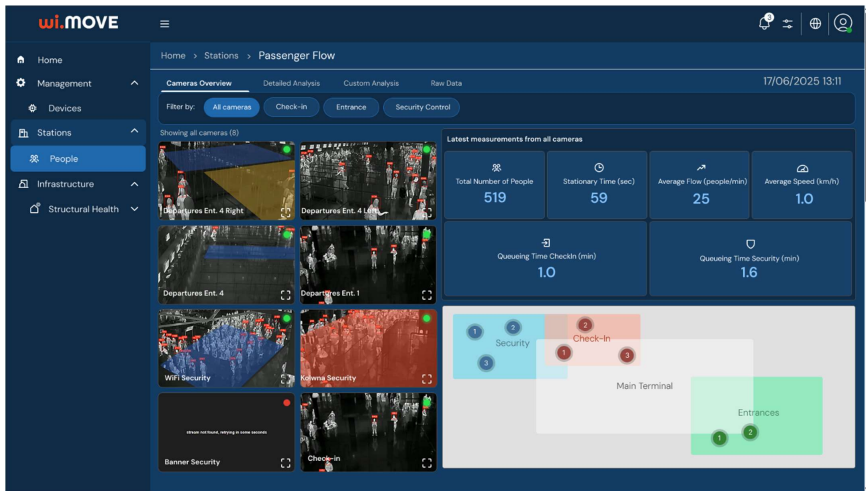
\includegraphics[width=0.7\textwidth]{figuras/antecedentes/antecedente-1.png}
\caption{Framework de seguimiento multiobjeto basado en centroides.}
\label{fig:ant1}
\end{figure}

\subsection{Antecedente 2: Video-Based Pedestrian Grouping Model Considering Long-Span Space~\cite{zhao2023}}

Zhao, Wang, Jia, Li, Dong y Ma publicaron en 2023, en el \textit{Journal
of Management Science and Engineering}, un modelo de agrupamiento de
peatones evaluado en el hall del Aeropuerto Internacional de Shanghai
Hongqiao.

\begin{itemize}
    \item \textbf{Problema abordado:} los pasajeros suelen viajar en
    grupos familiares o de amigos que no siempre permanecen juntos, sino
    que pueden separarse entre 2 y 12 metros al cruzar tiendas, columnas
    u otros pasajeros. Los trackers que tratan a cada persona como una
    entidad aislada fragmentan estos grupos y distorsionan las métricas
    de flujo y congestión.

    \item \textbf{Base de datos:} video CCTV real a 10~FPS del hall del
    aeropuerto, un entorno desafiante por su alta densidad, sus
    trayectorias cruzadas en horas pico y la iluminación natural variable
    de sus ventanales.

    \item \textbf{Metodología:} el pipeline tiene cuatro componentes:
    \begin{enumerate}
        \item \textbf{Proyección homográfica:} lleva cada detección al
        plano espacial común.
        \item \textbf{MIMTrack:} seguimiento multivista que mantiene
        trayectorias consistentes entre distintas cámaras del hall.
        \item \textbf{Sequential Pattern Analysis (SPA):} identifica
        similitudes de movimiento entre trayectorias cercanas en el
        tiempo.
        \item \textbf{Grafo de conectividad PGMSL:} estima la
        probabilidad de que dos trayectorias pertenezcan a personas que
        viajan juntas.
    \end{enumerate}

    \item \textbf{Resultados:} el sistema identifica tanto grupos
    compactos como grupos separados entre 2 y 12 metros, rango que los
    sistemas anteriores ignoraban. La detección de un grupo tomó en
    promedio entre 3.21 y 4.49 segundos, compatible con un monitoreo casi
    en tiempo real, y permite derivar métricas de comportamiento grupal,
    velocidad y congestión agregada.
\end{itemize}

De este antecedente se desprende que la similitud espacial y temporal
entre trayectorias, sin señales biométricas, basta para reconstruir
estructura significativa a nivel de grupo y de multitud. Esta idea
sustenta, en el sistema propuesto, el uso de Kernel Density Estimation
para hotspots y de PrefixSpan para rutas frecuentes, ambos calculados
solo a partir de coordenadas y marcas de tiempo asociadas a un
identificador seudónimo. Queda pendiente para trabajo futuro distinguir
entre viajeros individuales y grupos al calcular el tiempo de permanencia
y la tasa de captación por tienda.

\begin{figure}[!htbp]
\centering
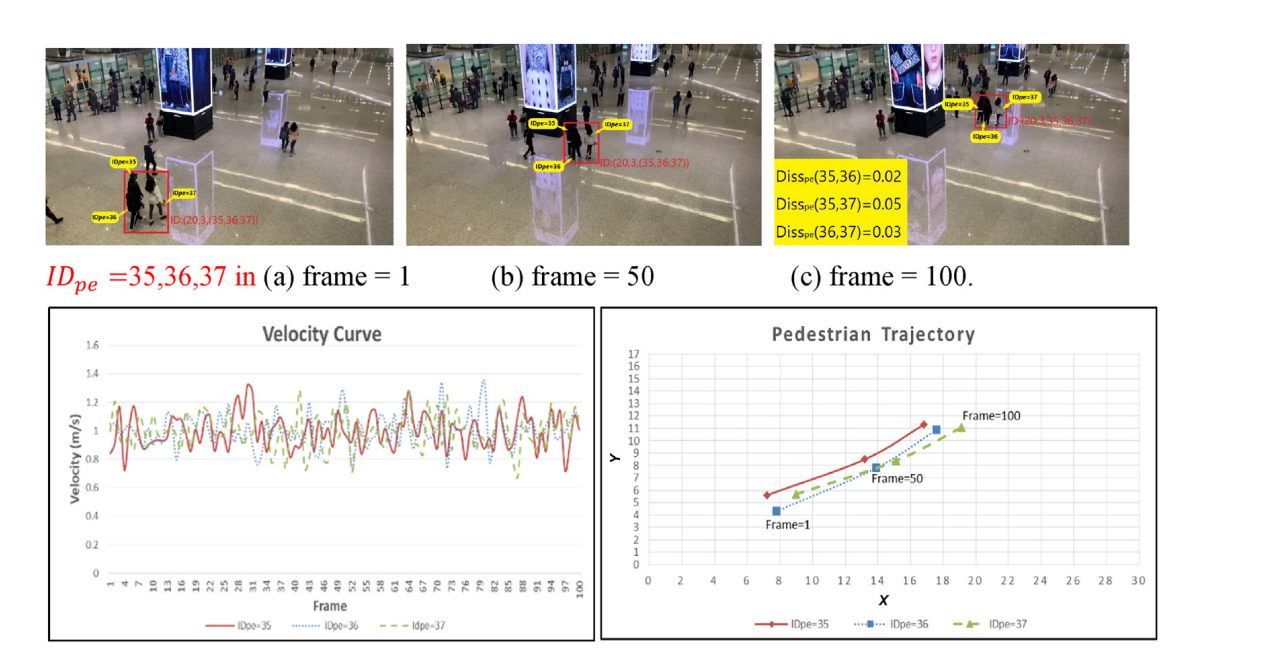
\includegraphics[width=0.7\textwidth]{figuras/antecedentes/antecedente-2.png}
\caption{Curva de velocidad y trayectoria de un grupo de tres peatones.}
\label{fig:ant2}
\end{figure}

\subsection{Antecedente 3: Multi-Camera Person Re-Identification Based on Trajectory Data~\cite{mendes2023}}

Mendes, Correia, Jorge, Brandão, Arriaga y Nunes publicaron en 2023, en
\textit{Applied Sciences}, un sistema de re-identificación multicámara
evaluado en un entorno comercial real durante siete días consecutivos.

\begin{itemize}
    \item \textbf{Problema abordado:} las cámaras existentes no comparten
    campo de visión, por lo que una misma persona recibe una identidad
    distinta en cada una; además, el reconocimiento facial es inviable
    por razones normativas y de aceptación social. Los autores proponen
    la re-identificación basada en trayectoria y apariencia como
    alternativa.

    \item \textbf{Base de datos:} 91 horas de video 1080p a 20~FPS,
    capturadas con cuatro cámaras durante siete días de operación real.

    \item \textbf{Metodología:} el pipeline tiene cuatro componentes:
    \begin{enumerate}
        \item \textbf{Detección con YOLOv5:} identifica personas en cada
        cuadro.
        \item \textbf{Tracking local con ByteTrack:} genera tracklets
        continuos por cámara.
        \item \textbf{Proyección homográfica:} lleva las posiciones a un
        plano común.
        \item \textbf{Re-identificación espacio-temporal:} combina la
        apariencia de cada tracklet con restricciones de tiempo y
        topología de cámaras, descartando asociaciones físicamente
        imposibles para no depender solo de la apariencia, que puede
        fallar ante cambios de iluminación o pose.
    \end{enumerate}

    \item \textbf{Resultados:} antes de la re-identificación había 512
    identidades, una por cada aparición en una cámara; después quedaron
    109 identidades globales frente a unas 76 personas reales, lo que
    equivale a un 82\,\% de re-identificaciones correctas y a una
    reducción de más de cuatro veces en el número de identidades.
\end{itemize}

Este es el precedente técnico más cercano al sistema propuesto, ya que
valida la combinación de un detector YOLO, un seguimiento local por
cámara y una re-identificación basada en apariencia y restricciones
espacio-temporales, que AeroVision implementa con el codificador
YOLO26s-ReID y una galería global compartida. Confirma además que el
enfoque es viable en un despliegue comercial real y respalda la decisión
de no procesar rasgos faciales. Su margen de error cercano al 18\,\%
muestra que la re-identificación sin biometría no es perfecta, por lo que
el sistema propuesto acumula muchas vistas por identidad, exige
coincidencia mutua y sin ambigüedad, y separa tracklets cuando una
fusión deja de ser coherente. La escala del experimento (cuatro cámaras,
91 horas) es, sin embargo, mucho menor que la de un aeropuerto completo.

\begin{figure}[!htbp]
\centering
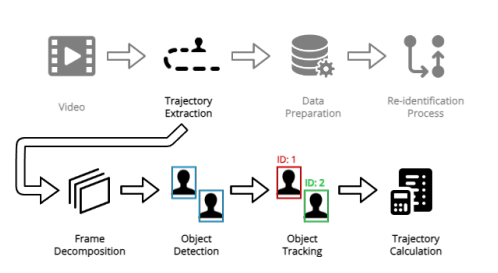
\includegraphics[width=0.7\textwidth]{figuras/antecedentes/antecedente-3.png}
\caption{Pipeline de extracción de trayectorias.}
\label{fig:ant3}
\end{figure}

\subsection{Antecedente 4: Pedestrian Attribute Recognition: MSP60K + LLM-PAR~\cite{jin2024}}

Jin, Wang, Zhu, Wang y Li publicaron en agosto de 2024, en la conferencia
AAAI, un dataset y un framework para el reconocimiento de atributos
peatonales en múltiples dominios.

\begin{itemize}
    \item \textbf{Problema abordado:} los datasets de atributos
    peatonales existentes, capturados en su mayoría en un único entorno
    controlado, generalizan mal cuando el sistema se despliega en otro
    dominio, por ejemplo al pasar de un centro comercial a un aeropuerto.

    \item \textbf{Base de datos:} MSP60K, con 60\,122 imágenes anotadas
    con 57 atributos (rango etario, género aparente, vestimenta,
    accesorios y postura), más de 5\,000 identidades y 8 escenarios
    heterogéneos, como obras de construcción, mercados, cocinas, colegios
    y espacios abiertos.

    \item \textbf{Metodología:} LLM-PAR tiene dos bloques:
    \begin{enumerate}
        \item \textbf{Codificador visual:} backbone EVA-ViT-G con un
        módulo LaRa, atención MEQFormer y bloques CBAM que refinan la
        representación de cada atributo.
        \item \textbf{Razonamiento semántico con LLM:} un modelo de
        lenguaje (Vicuna-7B u OPT-6.7B) razona sobre la compatibilidad
        entre atributos antes de la predicción final, por ejemplo,
        descartando la combinación de ``uniforme escolar'' y ``adulto
        mayor''.
    \end{enumerate}

    \item \textbf{Resultados:} F1 de 86.94 dentro del mismo dominio y
    F1 de 72.05 en evaluación entre dominios, una caída de más de 14
    puntos que los autores documentan explícitamente.
\end{itemize}

Para el sistema propuesto, este antecedente es relevante en la inferencia
demográfica aproximada: muestra que atributos generales como el rango
etario o el género aparente pueden estimarse a partir de la apariencia
corporal, sin reconocimiento facial, lo que resulta más compatible con la
Ley N.\textdegree~29733. En AeroVision esta idea se aplica, de forma
opcional, en la estimación de género por votación descrita en la
metodología. La caída de desempeño entre dominios es, sin embargo, una
advertencia: cualquier módulo demográfico deberá validarse con imágenes
del aeropuerto de Lima antes de asumir un desempeño equivalente.

\begin{figure}[!htbp]
\centering
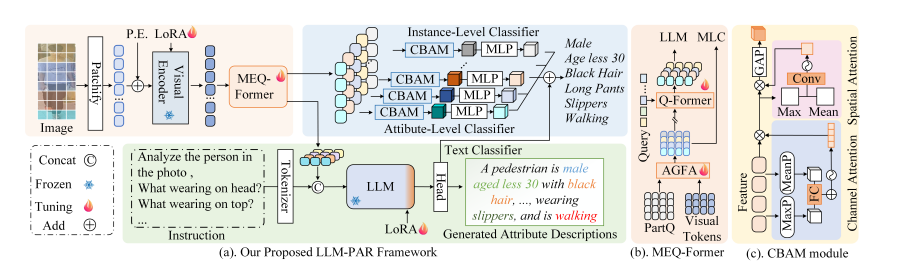
\includegraphics[width=0.7\textwidth]{figuras/antecedentes/antecedente-4.png}
\caption{Metodología de LLM-PAR.}
\label{fig:ant4}
\end{figure}

\subsection{Antecedente 5: A Unified Multi-view Multi-person Tracking Framework~\cite{yang2023}}

Yang et al., de Fujitsu Research (Japón), publicaron en 2023 un framework
unificado de tracking multivista y multipersona para generar trayectorias
globales en 3D o en vista superior a partir de varias cámaras.

\begin{itemize}
    \item \textbf{Problema abordado:} cuando cada cámara procesa sus
    detecciones sin un mecanismo de consistencia geométrica entre vistas,
    se obtienen trayectorias parciales e inconsistentes del recorrido
    real de una persona.

    \item \textbf{Base de datos:} WILDTRACK, MMPTRACK, Campus y Shelf,
    con escenas de hasta 313 personas simultáneas, 7 cámaras y más de 9.6
    horas de grabación.

    \item \textbf{Metodología:} el pipeline tiene cuatro componentes:
    \begin{enumerate}
        \item \textbf{YOLOX:} detector de personas por cámara.
        \item \textbf{Tracklets 2D por vista:} trayectorias locales
        independientes por cámara.
        \item \textbf{Distancia epipolar normalizada:} verifica si la
        posición observada en una cámara es geométricamente compatible
        con la observada en otra, dada su calibración.
        \item \textbf{PDNC y CMMT:} refinan la asociación final y la
        coherencia temporal de las trayectorias globales.
    \end{enumerate}

    \item \textbf{Resultados:} MOTA de 95.2\,\% e IDF1 de 97.5\,\% en
    WILDTRACK; MOTA de 95\,\% e IDF1 de 84.3\,\% a 67~FPS en MMPTRACK,
    entre los valores más altos de los antecedentes revisados.
\end{itemize}

Este antecedente valida la etapa de mapeo sobre un plano común: la
verificación geométrica entre vistas complementa la asociación por
apariencia al unificar detecciones de varias cámaras. Sus altos valores
de MOTA e IDF1 en escenas con más de 300 personas respaldan la
factibilidad de un seguimiento multicámara de calidad en horas pico. No
obstante, WILDTRACK y MMPTRACK son espacios relativamente controlados,
distintos de una terminal con mobiliario, equipaje y señalética, por lo
que el sistema propuesto debe validar estas métricas con datos propios.
En AeroVision, este tipo de verificación geométrica se activa en el modo
calibrado, cuando las homografías de las cámaras están validadas.

\begin{figure}[!htbp]
\centering
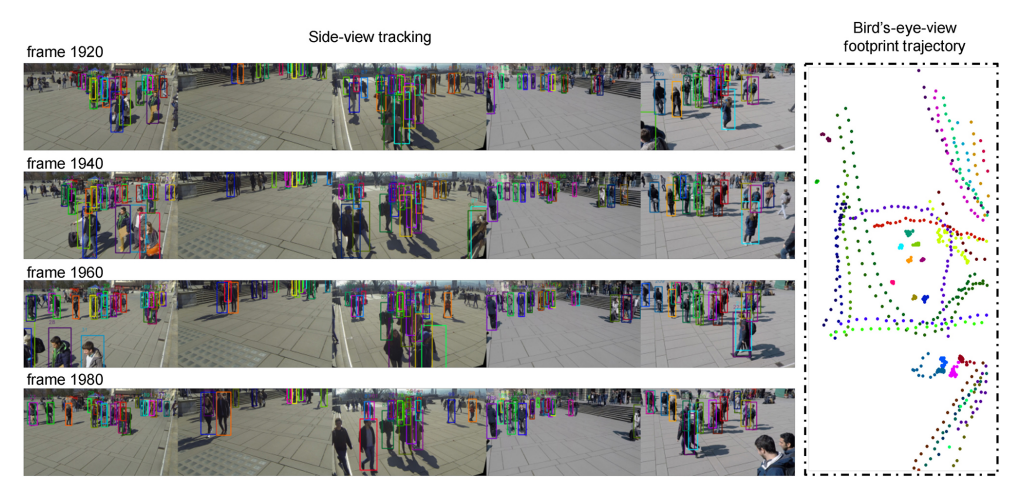
\includegraphics[width=0.7\textwidth]{figuras/antecedentes/antecedente-5.png}
\caption{Resultados del tracking en el conjunto de prueba.}
\label{fig:ant5}
\end{figure}

\subsection{Antecedente 6: Event Detection in Videos: A Framework for the Development of New Methods~\cite{zakharova2026}}

Zakharova, Bouwmans, Cioppa y colaboradores, de La Rochelle University y
otras instituciones, publicaron en arXiv, en julio de 2026, un framework
general para definir y evaluar eventos detectados en video.

\begin{itemize}
    \item \textbf{Problema abordado:} cada sistema de detección de
    eventos define ``evento'' a su manera y lo evalúa con métricas
    propias, lo que impide comparar métodos.

    \item \textbf{Base de datos:} FSD, con 43 cámaras IP y 153\,191
    cuadros anotados con máscaras de primer plano, y SUC, con 187\,500
    cuadros de 6 cámaras, ambos con peatones en movimiento, cambios
    bruscos de iluminación, objetos pequeños y visión nocturna.

    \item \textbf{Metodología:} se propone evaluar la detección de
    eventos en tres niveles:
    \begin{enumerate}
        \item \textbf{Píxel:} si cada píxel se clasificó correctamente
        como parte de un evento.
        \item \textbf{Cuadro:} si el cuadro completo refleja el evento
        esperado.
        \item \textbf{Segmento temporal:} si el evento se detecta a lo
        largo de una ventana de tiempo.
    \end{enumerate}
    En cada nivel se calculan precisión, recall, F1 e IoU de forma
    estandarizada.

    \item \textbf{Resultados:} en lugar de un único valor de desempeño,
    el trabajo valida el propio framework sobre FSD y SUC y demuestra que
    la evaluación multigranular es aplicable de forma consistente.
\end{itemize}

El motor de eventos del sistema propuesto (EXPOSURE, ENTER, DWELL, EXIT,
RETURN y QUEUE) se beneficia de este criterio: conviene evaluar cada tipo
de evento en distintas granularidades temporales en lugar de reportar una
sola métrica agregada, especialmente ante la iluminación variable y los
objetos pequeños propios de una terminal. Por su publicación reciente,
estas métricas aún no tienen adopción amplia, por lo que su uso en este
trabajo es una decisión metodológica temprana.

\begin{figure}[!htbp]
\centering
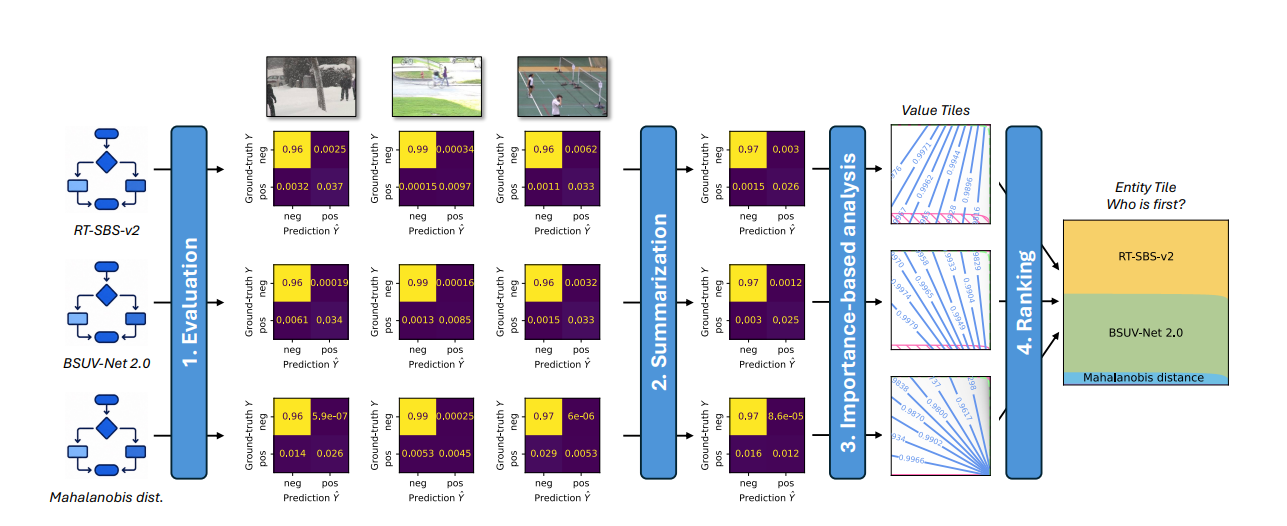
\includegraphics[width=0.7\textwidth]{figuras/antecedentes/antecedente-6.png}
\caption{Pipeline de evaluación de eventos.}
\label{fig:ant6}
\end{figure}

\subsection{Antecedente 7: Beyond Social Distancing: Application of Real-World Coordinates in a Multi-Camera System with Privacy Protection~\cite{ryan2023}}

Ryan y su equipo, de Stanford University, publicaron en 2023 un sistema
multicámara evaluado en un aeropuerto operativo de Dublín.

\begin{itemize}
    \item \textbf{Problema abordado:} construir una representación
    espacial unificada del movimiento de las personas en la terminal sin
    identificadores biométricos ni reconocimiento facial, dado que el
    sistema opera sobre CCTV en producción con pasajeros que no dieron
    consentimiento explícito.

    \item \textbf{Base de datos:} CCTV real de un aeropuerto de Dublín;
    el trabajo no especifica las horas de video ni el número de cámaras
    de la evaluación.

    \item \textbf{Metodología:} el pipeline tiene cuatro componentes:
    \begin{enumerate}
        \item \textbf{YOLOv5x:} detección de personas.
        \item \textbf{DeepSORT:} seguimiento local por cámara.
        \item \textbf{Transformación de perspectiva:} proyección sobre un
        plano común.
        \item \textbf{Re-identificación por distancia coseno:} asignación
        entre tracklets de distintas cámaras con el algoritmo húngaro.
    \end{enumerate}

    \item \textbf{Resultados:} trayectorias globales consistentes entre
    cámaras, integradas con un sistema GIS del aeropuerto, y una
    validación cualitativa, sin métricas cuantitativas de MOTA o IDF1.
\end{itemize}

Este antecedente fue evaluado en un aeropuerto real, por lo que confirma
que la combinación de detección, seguimiento local, proyección y
re-identificación sin biometría es viable en este dominio. Respalda la
proyección de las posiciones sobre un plano 2D común del aeropuerto Jorge
Chávez y su integración con un mapa. La ausencia de métricas
cuantitativas deja una laguna que el sistema propuesto busca cubrir
reportando precisión, recall e IDF1 con datos etiquetados.

\begin{figure}[!htbp]
\centering
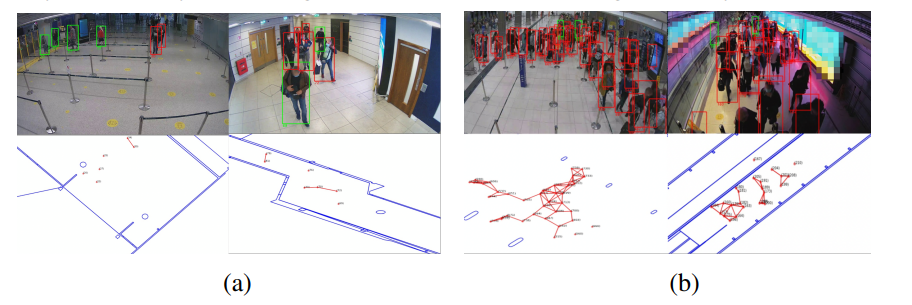
\includegraphics[width=0.7\textwidth]{figuras/antecedentes/antecedente-7.png}
\caption{a) Casos de éxito; b) casos fallidos por exceso de personas.}
\label{fig:ant7}
\end{figure}

\subsection{Antecedente 8: Fusion of CCTV Video and Spatial Information for Automated Crowd Congestion Monitoring in Public Urban Spaces~\cite{wonglaw2023}}

Wong y Law, también de Stanford University, publicaron en 2023 un sistema
que fusiona video CCTV con información espacial del entorno.

\begin{itemize}
    \item \textbf{Problema abordado:} la mayoría de sistemas de monitoreo
    de multitudes reporta solo la densidad instantánea por cámara, sin
    una vista agregada del espacio ni capacidad para predecir la
    congestión de los minutos siguientes.

    \item \textbf{Base de datos:} datos de Grand Central Station y del
    Stanford Stadium, con 17\,682 trayectorias sobre 6\,000 cuadros.

    \item \textbf{Metodología:} el pipeline tiene cinco componentes:
    \begin{enumerate}
        \item \textbf{YOLOv7-tiny:} detección de personas.
        \item \textbf{DeepSORT:} seguimiento local.
        \item \textbf{Homografía:} proyección sobre el plano del espacio.
        \item \textbf{CMGraph:} grafo de conectividad entre zonas.
        \item \textbf{GCN + GRU:} modelado temporal del flujo entre zonas
        para predecir la congestión futura.
    \end{enumerate}

    \item \textbf{Resultados:} MOTA de 73.7\,\%, MODA de 81.2\,\%, recall
    de 86.2\,\%, precisión de 94.6\,\%, y predicción de flujo con MSE de
    0.258 y MAE de 0.354; su tracking es más modesto que el de Yang et
    al.~\cite{yang2023}, pero es el único antecedente con capacidad
    predictiva.
\end{itemize}

Este antecedente aporta directamente al módulo de flujo entre zonas del
sistema propuesto. Representar el espacio como un grafo de zonas
conectadas permite generar mapas de calor y métricas de flujo, y admite
la predicción de congestión, que queda como trabajo futuro, ya que el
sistema propuesto reporta por ahora la congestión observada.

\begin{figure}[!htbp]
\centering
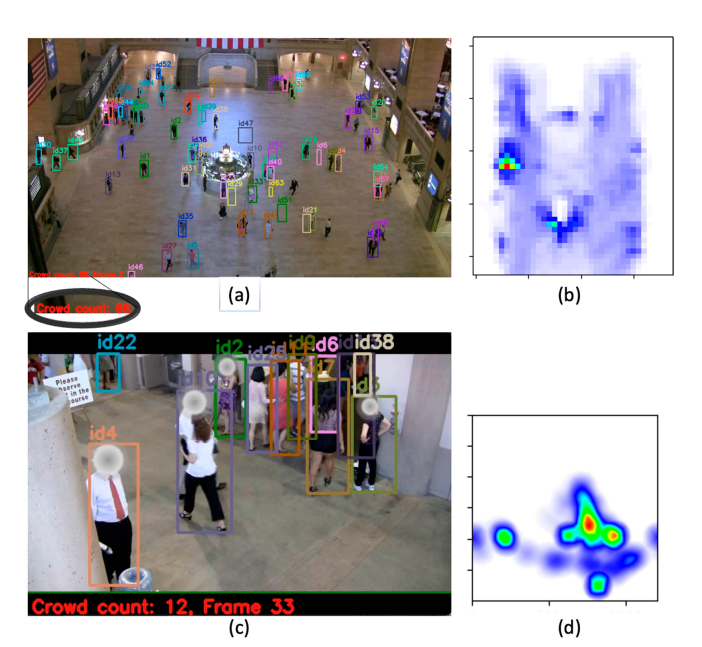
\includegraphics[width=0.7\textwidth]{figuras/antecedentes/antecedente-8.png}
\caption{Visualización de aglomeraciones en la estación.}
\label{fig:ant8}
\end{figure}

\subsection{Antecedente 9: Real-Time Pedestrian Detection and Multi-Object Tracking in Complex Airport Scenes via Frequency-Aware and Mamba-Enhanced Representation~\cite{zhou2026}}

Zhou y su equipo, en colaboración entre Chongqing y Nanjing Airlines
(China), publicaron en 2026 un tracker especializado para escenas
aeroportuarias.

\begin{itemize}
    \item \textbf{Problema abordado:} los trackers genéricos, evaluados
    sobre escenas urbanas o de vigilancia convencional, pierden
    desempeño en terminales aeroportuarias, donde la densidad, el
    equipaje, los cambios de iluminación y las oclusiones son más
    adversos que en los benchmarks estándar.

    \item \textbf{Base de datos:} AirportPassenger, dataset privado con
    12\,000 imágenes y 285\,000 instancias anotadas de pasajeros en
    escenas aeroportuarias reales.

    \item \textbf{Metodología:} AirMOTR incorpora dos componentes:
    \begin{enumerate}
        \item \textbf{Representaciones sensibles a la frecuencia:}
        capturan texturas y bordes que ayudan a distinguir personas entre
        equipaje y mobiliario.
        \item \textbf{Bloques Mamba:} modelos de espacio de estados, más
        eficientes que la atención estándar, para dependencias temporales
        largas.
    \end{enumerate}
    El modelo se comparó con DeepSORT, ByteTrack, BoT-SORT y MOTR sobre
    el mismo dataset.

    \item \textbf{Resultados:} AirMOTR obtuvo MOTA de 79.6\,\%, IDF1 de
    84.2\,\% y 41.6~FPS, superando a ByteTrack, segundo mejor, con MOTA
    de 72.3\,\%, IDF1 de 76.82\,\% y 42.5~FPS.
\end{itemize}

Este es el antecedente más cercano al dominio de aplicación, pues fue
evaluado en escenas aeroportuarias complejas. Muestra que los trackers
genéricos, incluido ByteTrack, ofrecen un desempeño sólido pero
mejorable en este dominio. La diferencia de 7.3 puntos de MOTA sugiere
que migrar a una arquitectura especializada no sería decisivo a corto
plazo, lo que justifica un seguidor local liviano cuya asociación en dos
etapas se inspira en ByteTrack, reforzado con apariencia corporal y
memoria visual para los cruces y oclusiones. La evaluación de
arquitecturas como AirMOTR queda como trabajo futuro, cuando se disponga
de suficientes datos propios.

\begin{figure}[!htbp]
\centering
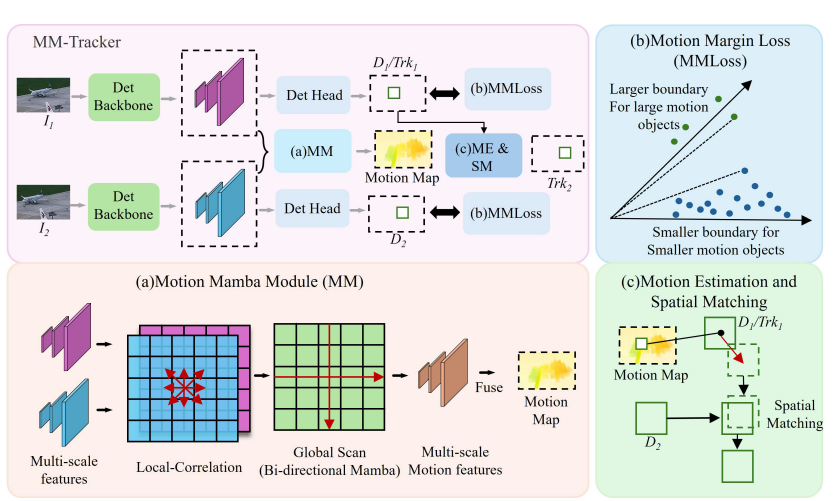
\includegraphics[width=0.7\textwidth]{figuras/antecedentes/antecedente-9.png}
\caption{Estructura del pipeline de seguimiento.}
\label{fig:ant9}
\end{figure}

\subsection{Cuadro Comparativo de Antecedentes}

El Cuadro~\ref{tab:antecedentes} resume las métricas principales, el
dominio de evaluación y el aporte de cada antecedente al sistema
propuesto.

\begin{table}[!htbp]
\centering
\caption{Resumen comparativo de los nueve antecedentes revisados.}
\label{tab:antecedentes}
\footnotesize
\begin{tabular}{@{}L{0.18\textwidth}L{0.17\textwidth}L{0.17\textwidth}L{0.38\textwidth}@{}}
\toprule
\textbf{Antecedente} & \textbf{Dominio de evaluación} & \textbf{Métrica clave} & \textbf{Aporte al sistema propuesto} \\
\midrule
Giannopoulou et al.~\cite{giannopoulou2026} & Aeropuerto real (Atenas) & mAP 0.87; 100\,\% de fiabilidad & Respalda un detector YOLO y un seguimiento local liviano en arquitectura modular \\
Zhao et al.~\cite{zhao2023} & Aeropuerto real (Shanghai) & Detección de grupo en 3.21--4.49~s & Sustenta KDE y PrefixSpan en la minería de patrones \\
Mendes et al.~\cite{mendes2023} & Entorno comercial real & 82\,\% de re-ID correcta & Precedente directo de la re-identificación multicámara sin rostro \\
Jin et al.~\cite{jin2024} & 8 dominios (MSP60K) & F1 86.94 / 72.05 entre dominios & Habilita inferencia demográfica sin biometría \\
Yang et al.~\cite{yang2023} & WILDTRACK / MMPTRACK & MOTA 95.2\,\% & Valida la verificación geométrica sobre un plano común \\
Zakharova et al.~\cite{zakharova2026} & FSD / SUC (CCTV real) & Evaluación multigranular & Criterio para evaluar el motor de eventos \\
Ryan et al.~\cite{ryan2023} & Aeropuerto real (Dublín) & Cualitativo (sin MOTA) & Valida la arquitectura completa en el dominio aeroportuario \\
Wong y Law~\cite{wonglaw2023} & Grand Central / Stanford Stadium & MOTA 73.7\,\%; MSE 0.258 & Grafo origen-destino y predicción de congestión futura \\
Zhou et al.~\cite{zhou2026} & Aeropuerto (AirportPassenger) & MOTA 79.6\,\% (AirMOTR) & Referencia para especializar el seguimiento local \\
\bottomrule
\end{tabular}
\end{table}

\FloatBarrier

\subsection{Síntesis y Vacío de Investigación}

Tomados en conjunto, los nueve antecedentes muestran que cada pieza
técnica del problema (detección, seguimiento, re-identificación sin
biometría, mapeo espacial, minería de patrones e insights comerciales) ha
sido resuelta por separado, varias veces incluso en aeropuertos reales
(Atenas, Shanghai Hongqiao, Dublín y las escenas de AirportPassenger),
pero ningún trabajo las integra en un solo pipeline desplegable bajo un
marco ético adecuado al contexto regulatorio latinoamericano.

El vacío que aborda este trabajo es, por tanto, más amplio que el de
cualquier antecedente aislado, pero más concreto que el de un sistema
comercial genérico. La predicción de
congestión, la especialización del seguimiento con arquitecturas tipo
AirMOTR y el clasificador de edad para la exclusión de menores no se
presentan como componentes implementados, sino como trabajo futuro.

\section{Especificación de Requerimientos}

\subsection{Casos de Uso del Sistema}

Esta sección presenta los casos de uso del sistema, que describen cómo cada
actor interactúa con las funciones definidas en los requerimientos
funcionales. Cada caso de uso indica su actor principal, el requerimiento
que cubre, su historia de usuario, precondiciones, flujo principal, flujos
alternativos y postcondiciones. El sistema tiene dos actores: el
\textbf{Usuario comercial}, que consulta el análisis y los insights, y el
\textbf{Usuario administrador}, que monitorea, configura el mapa y procesa
los videos. Los casos de uso describen el sistema objetivo; en el prototipo,
el inicio de sesión (CU-01) es de demostración y no distingue roles.

\textbf{CU-01: Iniciar y cerrar sesión}

\textbf{Actor principal:} Usuario comercial, Usuario administrador \\
\textbf{Requerimiento:} RF-01

\textbf{Historia de usuario:} Como usuario del sistema, quiero iniciar sesión con mis credenciales y cerrarla al terminar, para acceder de forma segura solo a las funciones permitidas por mi rol.

\textbf{Precondiciones:} El usuario está registrado y activo.

\textbf{Flujo principal:}
\begin{enumerate}
    \item El usuario ingresa su usuario y contraseña.
    \item El sistema valida las credenciales y el rol.
    \item El sistema redirige a la vista permitida para su rol.
    \item Al pulsar ``Cerrar sesión'', el sistema invalida la sesión.
\end{enumerate}

\textbf{Flujos alternativos:} Si las credenciales son inválidas, el sistema
muestra un error; tras varios intentos fallidos, bloquea el acceso
temporalmente.

\textbf{Postcondiciones:} Sesión activa con los permisos del rol, o sesión cerrada.

\begin{figure}[!htbp]
\centering
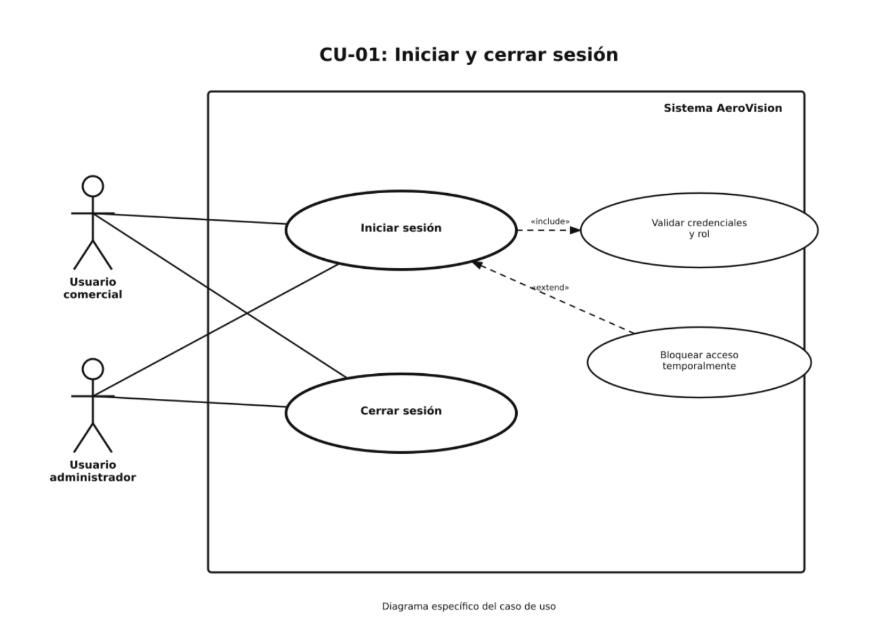
\includegraphics[width=0.6\linewidth]{figuras/casos-de-uso/cu-01.png}
\caption{CU-01: Iniciar y cerrar sesión}
\label{fig:cu01}
\end{figure}

\textbf{CU-02: Monitorear personas y trayectorias en vivo}

\textbf{Actor principal:} Usuario administrador \\
\textbf{Requerimiento:} RF-02

\textbf{Historia de usuario:} Como usuario administrador, quiero visualizar en tiempo real a las personas y sus trayectorias sobre el plano del aeropuerto, para conocer el estado de la operación y actuar ante aglomeraciones o incidencias.

\textbf{Precondiciones:} Sesión iniciada, plano y zonas configurados, y
trayectorias disponibles.

\textbf{Flujo principal:}
\begin{enumerate}
    \item El usuario accede a la pantalla ``En vivo''.
    \item El sistema muestra el plano 2D con las personas, su estado y su zona.
    \item El usuario activa las capas de trayectorias, zonas o cámaras.
    \item El usuario selecciona una persona.
    \item El sistema aísla su recorrido y sus eventos.
\end{enumerate}

\textbf{Flujos alternativos:} Si no hay datos en la ventana, el sistema
muestra el aviso ``sin observaciones''.

\textbf{Postcondiciones:} Estado actual del aeropuerto visible con
identificadores seudónimos.

\begin{figure}[!htbp]
\centering
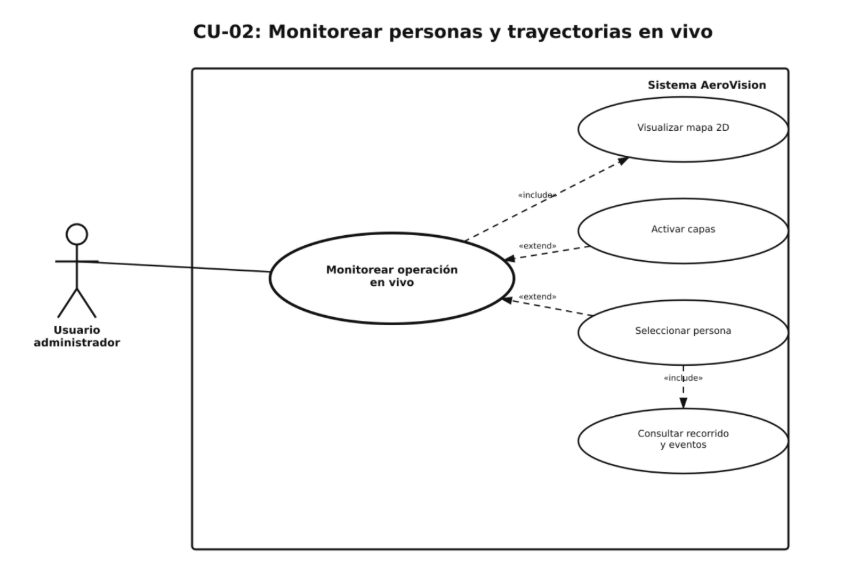
\includegraphics[width=0.6\linewidth]{figuras/casos-de-uso/cu-02.png}
\caption{CU-02: Monitorear personas y trayectorias en vivo}
\label{fig:cu02}
\end{figure}

\textbf{CU-03: Reproducir histórico de movimiento}

\textbf{Actor principal:} Usuario comercial, Usuario administrador \\
\textbf{Requerimiento:} RF-04

\textbf{Historia de usuario:} Como usuario del sistema, quiero reproducir el movimiento histórico de las personas en un periodo específico, para entender cómo se comportó el flujo en un momento pasado.

\textbf{Precondiciones:} Existen posiciones registradas en el periodo.

\textbf{Flujo principal:}
\begin{enumerate}
    \item El usuario elige la ventana temporal.
    \item El sistema carga la reproducción.
    \item El usuario reproduce, pausa, arrastra la línea de tiempo o cambia la velocidad.
    \item El sistema recalcula los indicadores en el instante reproducido.
\end{enumerate}

\textbf{Flujos alternativos:} Si el filtro es inválido, el sistema lo
rechaza con un mensaje.

\textbf{Postcondiciones:} Movimiento del periodo reproducido junto con sus métricas.

\begin{figure}[!htbp]
\centering
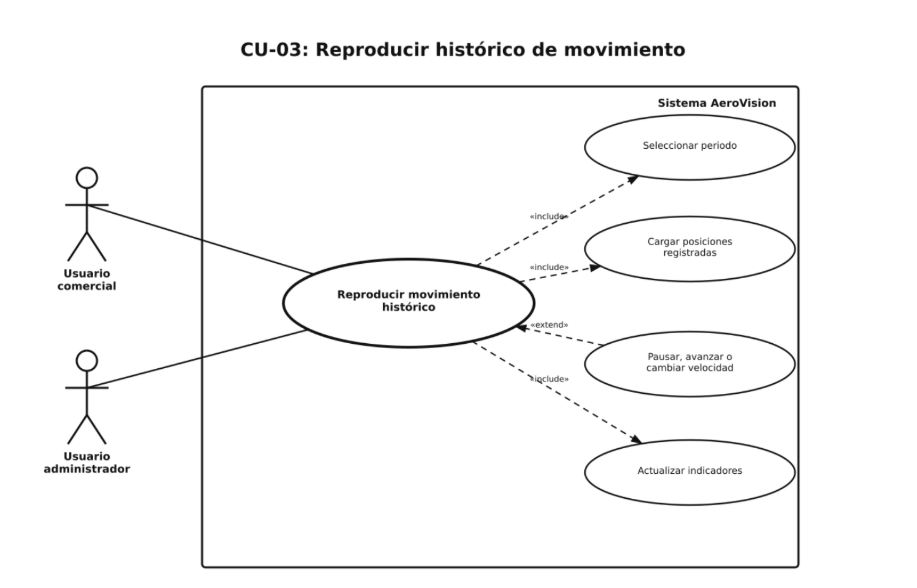
\includegraphics[width=0.6\linewidth]{figuras/casos-de-uso/cu-03.png}
\caption{CU-03: Reproducir histórico de movimiento}
\label{fig:cu03}
\end{figure}

\textbf{CU-04: Configurar zonas del mapa}

\textbf{Actor principal:} Usuario administrador \\
\textbf{Requerimiento:} RF-03

\textbf{Historia de usuario:} Como usuario administrador, quiero crear, modificar y eliminar zonas sobre el plano, para reflejar en el sistema la distribución real de puestos y áreas del aeropuerto.

\textbf{Precondiciones:} Sesión de usuario administrador en la pantalla ``Configuración''.

\textbf{Flujo principal:}
\begin{enumerate}
    \item El usuario pulsa ``Editar'' y luego ``+ Zona''.
    \item El usuario marca los vértices sobre el plano y pulsa ``Terminar zona''.
    \item El usuario define nombre, tipo, color y, si es INTERIOR o FRONTAGE, su local.
    \item El sistema valida la geometría y registra la zona.
\end{enumerate}

\textbf{Flujos alternativos:} Si cancela, se descarta el borrador. Si la
geometría es inválida, el sistema rechaza el cambio. Para quitar una zona,
el usuario pulsa ``Eliminar zona''.

\textbf{Postcondiciones:} Zona disponible en el mapa y en los insights.

\begin{figure}[!htbp]
\centering
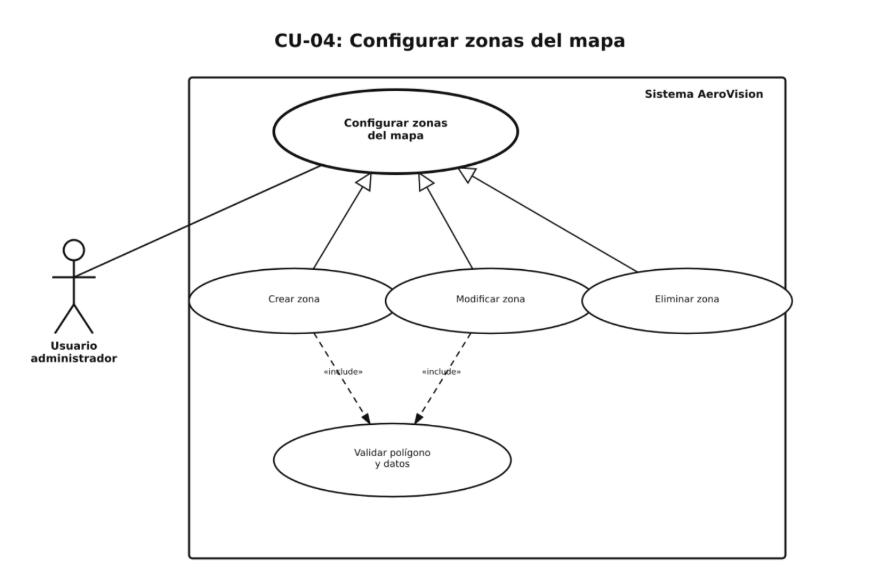
\includegraphics[width=0.6\linewidth]{figuras/casos-de-uso/cu-04.png}
\caption{CU-04: Configurar zonas del mapa}
\label{fig:cu04}
\end{figure}
\textbf{CU-05: Configurar cámaras y cobertura}

\textbf{Actor principal:} Usuario administrador \\
\textbf{Requerimiento:} RF-03

\textbf{Historia de usuario:} Como usuario administrador, quiero ubicar y orientar las cámaras en el plano, para que el sistema sepa qué zona física observa cada una.

\textbf{Precondiciones:} Sesión de usuario administrador en la pantalla ``Configuración''.

\textbf{Flujo principal:}
\begin{enumerate}
    \item El usuario pulsa ``Editar'' y luego ``+ Cámara'', y marca su ubicación.
    \item El usuario define su nombre, su posición (X, Y) y su dirección.
    \item El usuario arrastra la cámara para moverla y su círculo para girarla; el plano muestra su campo de visión.
    \item El sistema guarda la pose al soltarla.
\end{enumerate}

\textbf{Flujos alternativos:} Una cámara con trayectorias no se puede
eliminar. Volver a publicar el Build no reemplaza una pose ajustada a mano.

\textbf{Postcondiciones:} Cámara registrada en el plano con su posición y
dirección.

\begin{figure}[!htbp]
\centering
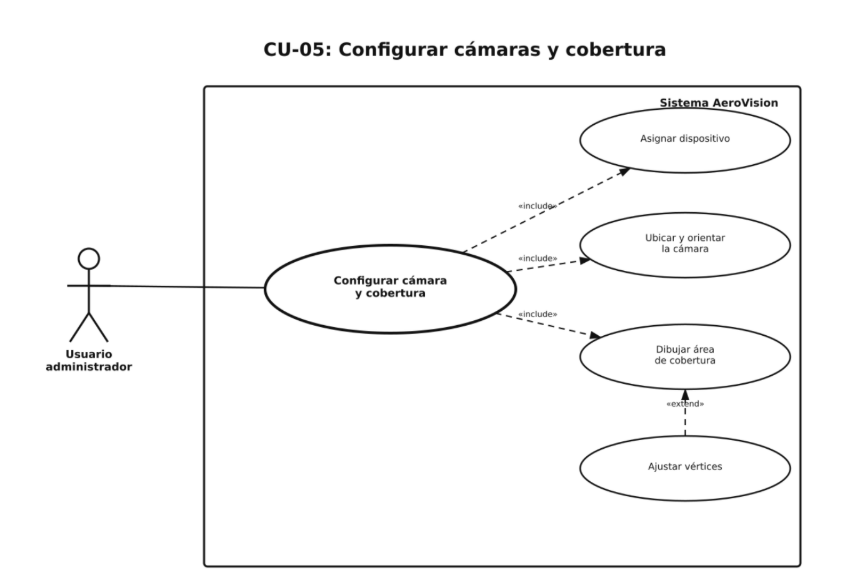
\includegraphics[width=0.6\linewidth]{figuras/casos-de-uso/cu-05.png}
\caption{CU-05: Configurar cámaras y cobertura}
\label{fig:cu05}
\end{figure}

\textbf{CU-06: Ver cámara en vivo}

\textbf{Actor principal:} Usuario administrador \\
\textbf{Requerimiento:} RF-02

\textbf{Historia de usuario:} Como usuario administrador, quiero ver en vivo lo que capta cada teléfono conectado como cámara, con las detecciones del modelo, para verificar directamente lo que ocurre en una zona.

\textbf{Precondiciones:} Teléfonos unidos desde la página de cámara.

\textbf{Flujo principal:}
\begin{enumerate}
    \item El usuario abre la pantalla ``Teléfonos''.
    \item El sistema muestra cada teléfono con las cajas, el ID y el género que publica el modelo.
    \item El usuario puede quitar un teléfono de la lista.
\end{enumerate}

\textbf{Flujos alternativos:} Si el modelo no está procesando, se ve el
video directo del teléfono.

\textbf{Postcondiciones:} El teléfono quitado deja de enviar video.

\begin{figure}[!htbp]
\centering
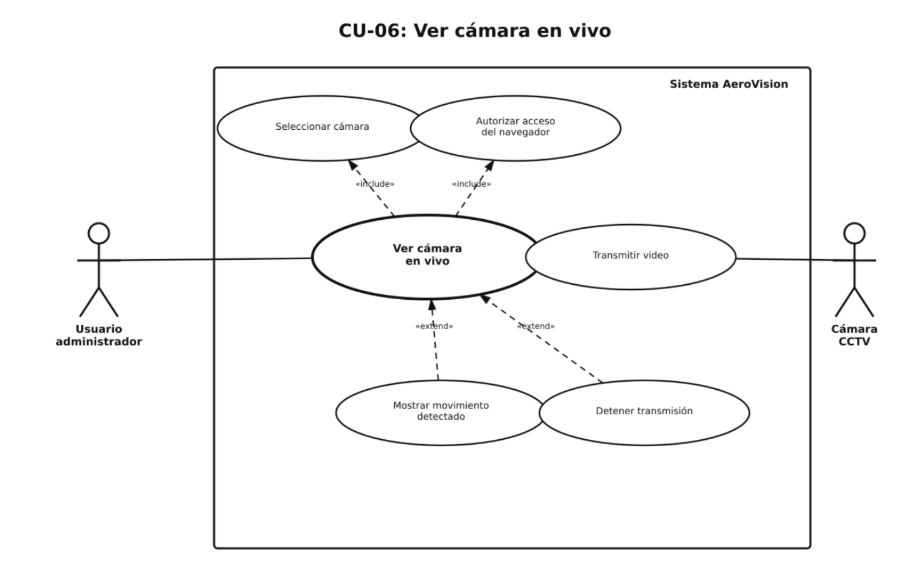
\includegraphics[width=0.6\linewidth]{figuras/casos-de-uso/cu-06.png}
\caption{CU-06: Ver cámara en vivo}
\label{fig:cu06}
\end{figure}

\textbf{CU-07: Consultar mapa de calor}

\textbf{Actor principal:} Usuario comercial \\
\textbf{Requerimiento:} RF-04

\textbf{Historia de usuario:} Como usuario comercial, quiero visualizar un mapa de calor de las zonas con mayor aglomeración en un periodo, para identificar los puntos de mayor tránsito y tomar decisiones comerciales informadas.

\textbf{Precondiciones:} Existen posiciones históricas registradas.

\textbf{Flujo principal:}
\begin{enumerate}
    \item El usuario accede a la pantalla ``Insights''.
    \item El usuario selecciona el periodo.
    \item El sistema superpone el mapa de calor sobre el plano con su leyenda.
\end{enumerate}

\textbf{Flujos alternativos:} Si el periodo no tiene datos, el sistema
muestra el mapa vacío con un aviso.

\textbf{Postcondiciones:} Zonas de mayor aglomeración identificadas.

\begin{figure}[!htbp]
\centering
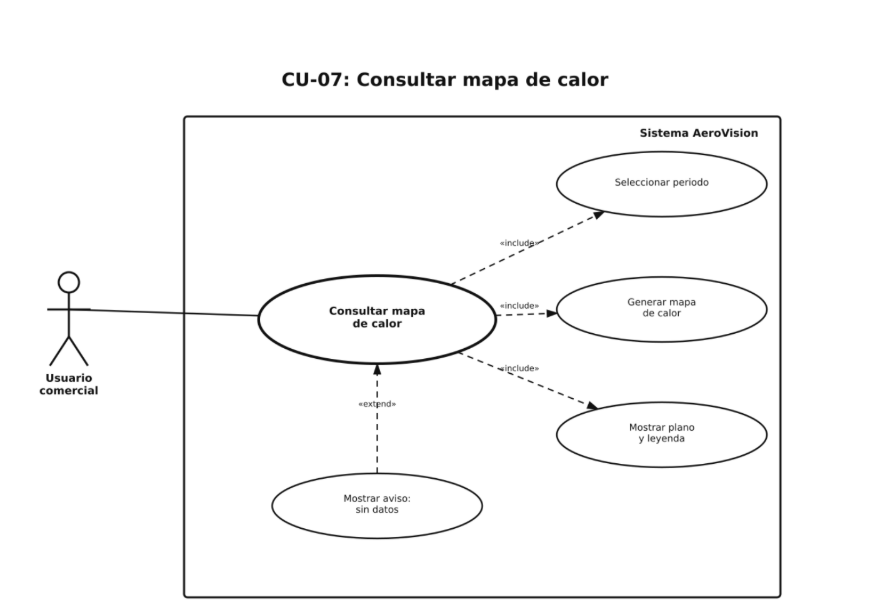
\includegraphics[width=0.6\linewidth]{figuras/casos-de-uso/cu-07.png}
\caption{CU-07: Consultar mapa de calor}
\label{fig:cu07}
\end{figure}

\textbf{CU-08: Consultar insights por zona}

\textbf{Actor principal:} Usuario comercial \\
\textbf{Requerimiento:} RF-05

\textbf{Historia de usuario:} Como usuario comercial, quiero consultar las visitas, la permanencia y la captación por zona y periodo, para evaluar el desempeño de cada punto comercial y comparar su evolución.

\textbf{Precondiciones:} Zonas configuradas y visitas registradas.

\textbf{Flujo principal:}
\begin{enumerate}
    \item El usuario accede a la pantalla ``Insights''.
    \item El usuario selecciona el periodo y la zona.
    \item El sistema muestra visitas, pass-by, permanencia, captación, densidad y su evolución en el tiempo.
\end{enumerate}

\textbf{Flujos alternativos:} El usuario puede comparar dos periodos.

\textbf{Postcondiciones:} Métricas agregadas por zona sin datos personales.

\begin{figure}[!htbp]
\centering
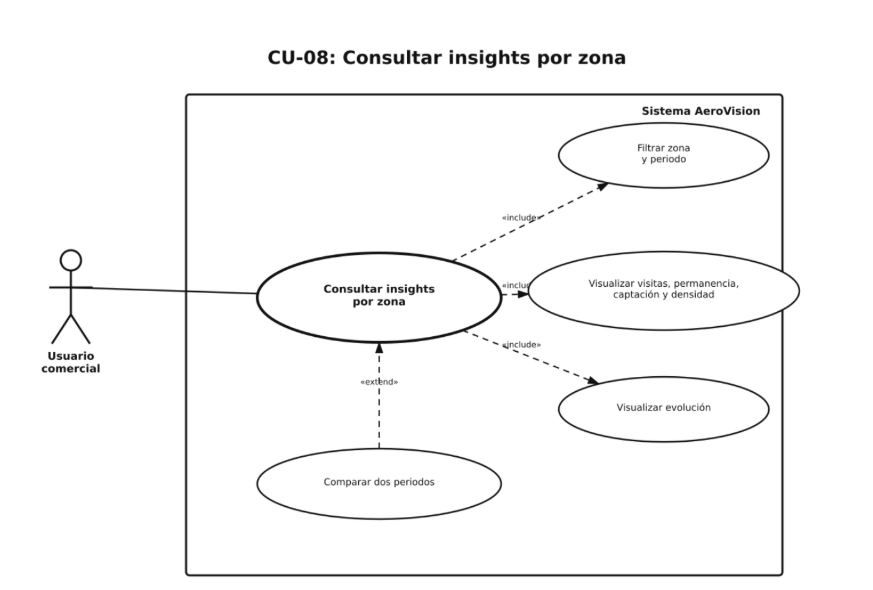
\includegraphics[width=0.6\linewidth]{figuras/casos-de-uso/cu-08.png}
\caption{CU-08: Consultar insights por zona}
\label{fig:cu08}
\end{figure}
\textbf{CU-09: Analizar flujos entre zonas}

\textbf{Actor principal:} Usuario comercial \\
\textbf{Requerimiento:} RF-04

\textbf{Historia de usuario:} Como usuario comercial, quiero visualizar los flujos de personas entre zonas y su volumen, para entender las rutas más frecuentes y optimizar la ubicación de los puntos comerciales.

\textbf{Precondiciones:} Existen entradas y salidas de zonas registradas.

\textbf{Flujo principal:}
\begin{enumerate}
    \item El usuario activa la capa de flujos.
    \item El sistema dibuja las transiciones de origen a destino con su volumen.
\end{enumerate}

\textbf{Flujos alternativos:} Si no hay transiciones en el periodo, el
sistema muestra un aviso.

\textbf{Postcondiciones:} Rutas más frecuentes entre zonas visibles.

\begin{figure}[!htbp]
\centering
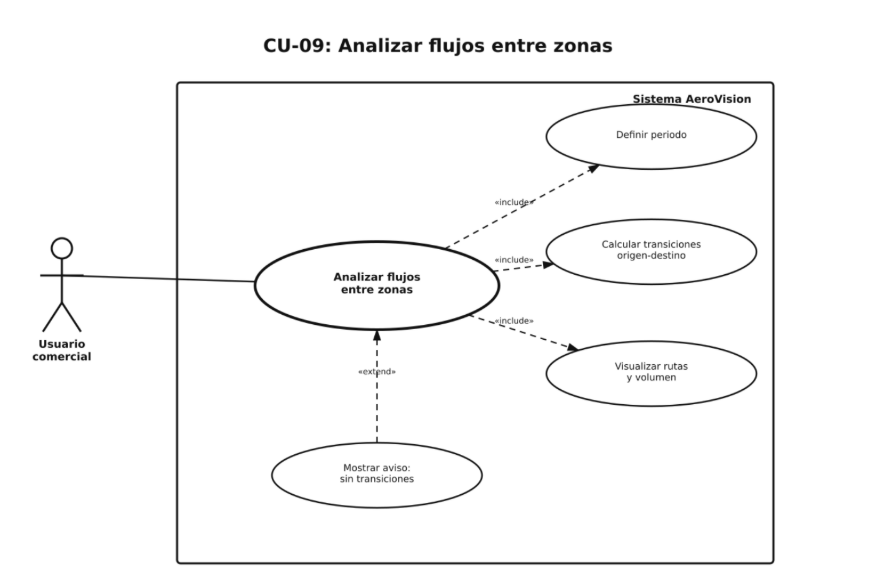
\includegraphics[width=0.6\linewidth]{figuras/casos-de-uso/cu-09.png}
\caption{CU-09: Analizar flujos entre zonas}
\label{fig:cu09}
\end{figure}

\textbf{CU-10: Exportar reporte}

\textbf{Actor principal:} Usuario comercial \\
\textbf{Requerimiento:} RF-05

\textbf{Historia de usuario:} Como usuario comercial, quiero exportar los insights de un periodo en CSV o PDF, para compartir los resultados con mi equipo o usarlos fuera del sistema.

\textbf{Precondiciones:} Insights cargados para un periodo.

\textbf{Flujo principal:}
\begin{enumerate}
    \item El usuario pulsa ``Exportar''.
    \item El usuario elige el formato CSV o PDF.
    \item El sistema genera y descarga el archivo.
\end{enumerate}

\textbf{Flujos alternativos:} Si la generación es prolongada, el sistema
muestra el progreso.

\textbf{Postcondiciones:} Reporte descargado.

\begin{figure}[!htbp]
\centering
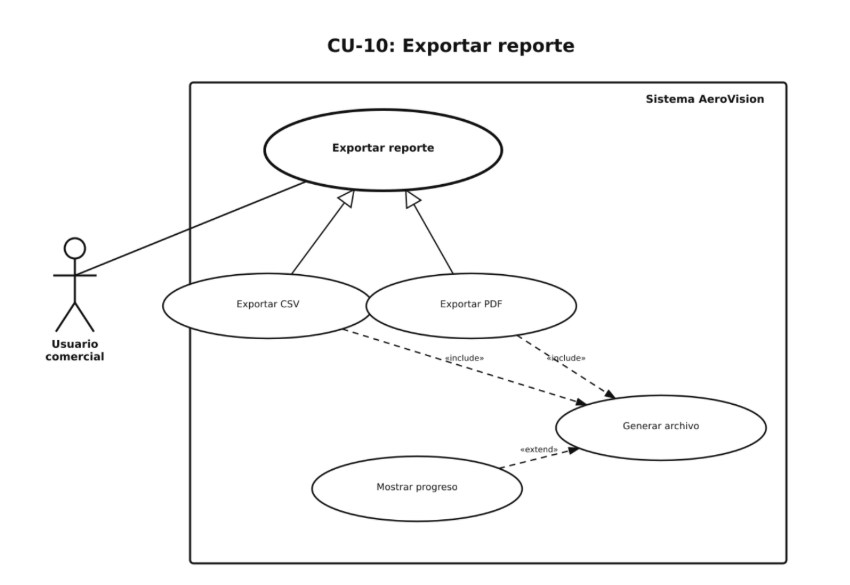
\includegraphics[width=0.6\linewidth]{figuras/casos-de-uso/cu-10.png}
\caption{CU-10: Exportar reporte}
\label{fig:cu10}
\end{figure}

\textbf{CU-11: Procesar videos multicámara}

\textbf{Actor principal:} Usuario administrador \\
\textbf{Requerimiento:} RF-06

\textbf{Historia de usuario:} Como usuario administrador, quiero que el sistema procese los videos de varias cámaras y siga a las personas de forma seudónima entre ellas, para obtener trayectorias completas sin identificar a nadie.

\textbf{Precondiciones:} Videos y configuración de cámaras disponibles.

\textbf{Flujo principal:}
\begin{enumerate}
    \item El usuario inicia el procesamiento de los videos.
    \item El sistema abre una sesión de análisis con su configuración y
    el manifiesto de los modelos.
    \item El sistema detecta y sigue a las personas en cada cámara.
    \item El sistema asocia a la misma persona entre cámaras.
    \item El sistema ubica cada posición en el plano.
    \item El sistema reconcilia las identidades y registra las
    trayectorias seudónimas.
\end{enumerate}

\textbf{Flujos alternativos:} Si una cámara no está calibrada, la
trayectoria se registra sin coordenadas en el plano. Si el usuario
interrumpe el procesamiento, se conserva y reconcilia lo procesado hasta
ese momento.

\textbf{Postcondiciones:} Trayectorias disponibles para el mapa y los insights.

\FloatBarrier

\begin{figure}[!htbp]
\centering
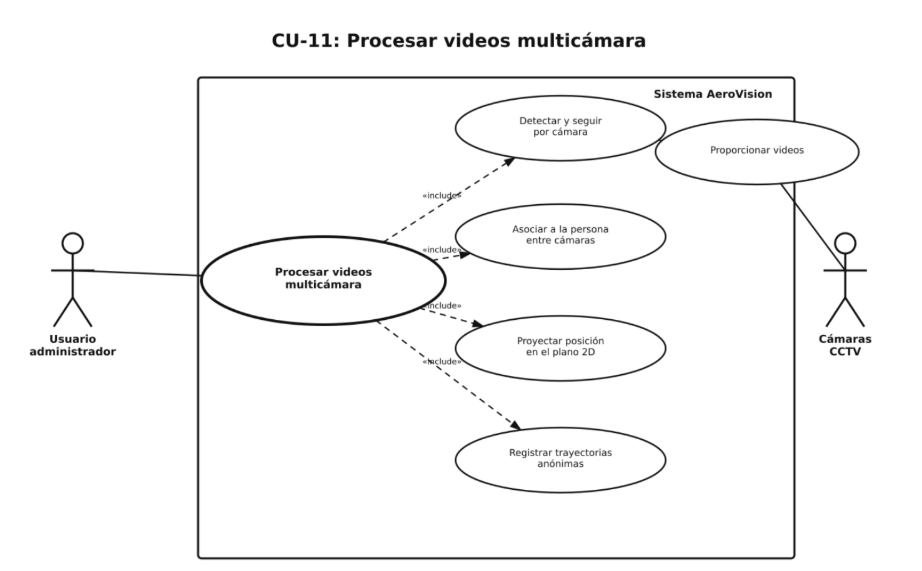
\includegraphics[width=0.6\linewidth]{figuras/casos-de-uso/cu-11.png}
\caption{CU-11: Procesar videos multicámara}
\label{fig:cu11}
\end{figure}
\subsection{Requerimientos Funcionales y No Funcionales}

\begin{table}[!htbp]
\caption{Requisitos Funcionales y No Funcionales}
\label{tab:requisitos}
\centering
\footnotesize
\setlength{\tabcolsep}{5pt}
\renewcommand{\arraystretch}{0.9}
\begin{tabular}{L{0.07\textwidth}L{0.12\textwidth}L{0.29\textwidth}L{0.41\textwidth}}
\hline
\textbf{ID} & \textbf{Tipo} & \textbf{Requisito} & \textbf{Criterio de aceptación / Verificación} \\
\hline
RF-01 & Funcional & Autenticación y control de acceso por roles & Solo usuarios autenticados acceden; el usuario comercial consulta y el usuario administrador además configura y procesa \\
RF-02 & Funcional & Monitoreo en vivo sobre el mapa 2D & Plano con personas seudónimas, estado, zona actual, trayectorias y video de las cámaras asignadas \\
RF-03 & Funcional & Personalización del mapa, cámaras y zonas & Ubicar y orientar cámaras y dibujar zonas con nombre, tipo y color; crear, modificar y eliminar con cambios persistentes \\
RF-04 & Funcional & Análisis histórico del movimiento & Reproducción temporal, mapa de calor y flujos entre zonas para un periodo filtrado \\
RF-05 & Funcional & Insights comerciales segmentados por zona & Visitas, pass-by, permanencia, captación y densidad por zona y periodo; exportables \\
RF-06 & Funcional & Seguimiento multicámara seudónimo de personas & Detectar y seguir personas, asociarlas entre cámaras sin reconocimiento facial, asignar identificador seudónimo y registrar trayectorias \\
RNF-01 & No Funcional & Seguridad & Conexión segura (HTTPS) y límite de peticiones por IP; contraseñas con hash y autorización por rol en el backend, previstas para producción \\
RNF-02 & No Funcional & Privacidad y normativa & Sin rostros, recortes ni video almacenados; identificadores seudónimos de sesión; vectores de apariencia solo en la memoria en vivo, borrados tras 7 días sin ver a la persona; cumplimiento de la Ley N.\textdegree~29733 \\
RNF-03 & No Funcional & Integridad de datos & Rechazo de cambios simultáneos conflictivos, de geometrías inválidas y de filas que violen las restricciones del esquema \\
RNF-04 & No Funcional & Rendimiento & Consultas y actualización del mapa en tiempos aceptables para la operación \\
RNF-05 & No Funcional & Fluidez de visualización & Animación continua y respuesta inmediata a la interacción \\
RNF-06 & No Funcional & Disponibilidad & Verificación de estado y recuperación automática ante fallos \\
RNF-07 & No Funcional & Portabilidad & Despliegue en contenedores; plano local sin servicios externos \\
RNF-08 & No Funcional & Usabilidad & Confirmación antes de borrar; interfaz aprendible sin capacitación extensa \\
RNF-09 & No Funcional & Mantenibilidad & API versionada, migraciones de base de datos versionadas y pruebas automatizadas \\
RNF-10 & No Funcional & Compatibilidad & Funcionamiento en navegadores modernos; cámara solo con conexión segura \\
RNF-11 & No Funcional & Precisión del seguimiento & Identidades consistentes dentro de cada cámara y entre cámaras, validadas con videos etiquetados \\
RNF-12 & No Funcional & Rendimiento del procesamiento de video & Procesamiento de varias cámaras simultáneas al ritmo del video \\
RNF-13 & No Funcional & Reproducibilidad & Pesos, configuración y versiones de dependencias registrados con huella SHA-256 en cada sesión de análisis \\
\hline
\end{tabular}
\end{table}

\FloatBarrier

\section{Metodología}

AeroVision propone una metodología de tres partes encadenadas para
transformar el video CCTV en trayectorias espaciales seudónimas y,
posteriormente, convertir esas trayectorias en indicadores operativos y
comerciales. En la primera parte se construye y estabiliza el seguimiento
local de personas dentro de cada cámara. En la segunda, los tracklets de
todas las cámaras se asocian mediante una galería global compartida,
reciben un identificador seudónimo y se proyectan sobre un plano 2D común
mediante homografía. En la tercera, las trayectorias históricas se
procesan para detectar zonas de concentración, rutas frecuentes, flujos
entre zonas y métricas de comportamiento.

El flujo metodológico general es:

\begin{equation}
\begin{aligned}
\text{CCTV}
&\rightarrow \text{Tracking local}
\rightarrow \text{Re-ID multicámara} \\
&\rightarrow \text{Mapeo 2D}
\rightarrow \text{Histórico} \\
&\rightarrow \text{Insights}.
\end{aligned}
\end{equation}

El núcleo metodológico está compuesto por YOLO26m para la detección de
personas; un seguidor local híbrido basado en movimiento, IoU, escala,
apariencia corporal (histogramas de color y ResNet18) y memoria visual;
el codificador YOLO26s-ReID con una galería global compartida para la
asociación entre cámaras; homografía para la proyección espacial; un
modelo CLIP local, opcional, para la estimación agregada de género;
PostGIS para el almacenamiento espacial; y Vue.js para la visualización.

Ningún modelo se entrena dentro del proyecto: todos los pesos son
preentrenados, se cargan desde disco sin descargas ni telemetría, y cada
ejecución exporta un manifiesto con la huella SHA-256 de los pesos, de la
configuración y del propio notebook, junto con las versiones de las
dependencias (PyTorch, Ultralytics, OpenCV, ONNX Runtime, entre otras).
Los umbrales del seguidor y de la asociación se guardan en dos archivos
versionados: uno para la detección y el seguimiento local, y otro para
el registro de cámaras y la asociación multicámara.

\subsection{Parte I: Construcción del seguimiento local}

La primera parte mantiene una identidad local estable mientras una
persona permanece en el campo de visión de una cámara. El seguimiento
debe conservar el identificador ante desplazamientos, cambios de
orientación, cruces entre personas, oclusiones parciales y pérdidas
breves de detección.

Cada cámara ejecuta una instancia independiente del seguidor y procesa
sus cuadros en orden temporal estrictamente creciente, sin omitir
ninguno, de modo que cada observación utiliza como contexto el estado
construido en los cuadros anteriores. El detector y el extractor de
apariencia se cargan una sola vez y se comparten entre cámaras. El
seguidor también se actualiza en los cuadros sin detecciones, para que
el tiempo de ausencia de cada track siga avanzando.

\subsubsection{Detección de personas}

Cada cuadro se procesa con YOLO26m restringido a la clase
\textit{person}, con una entrada de 640 píxeles. Cada detección se
representa como:

\begin{equation}
d_i = (x_1,y_1,x_2,y_2,c_i),
\end{equation}

donde $c_i$ es la confianza del detector. Para aprovechar la GPU, el
detector procesa en un mismo lote un cuadro de cada cámara
correspondiente al mismo instante, sin mezclar nunca cuadros de instantes
distintos. Se utiliza precisión completa (FP32), porque la media
precisión alteraba levemente las confianzas y, con ello, decisiones del
seguidor cercanas a los umbrales.

Las detecciones se aceptan desde una confianza de 0.30, que coincide con
el umbral de visualización, de modo que todo lo que se sigue también se
dibuja. Las detecciones de confianza baja se conservan, pero solo pueden
prolongar un track existente; nunca crean una identidad nueva. Este
criterio es deliberado: elevar solo el umbral del detector no reduce los
identificadores espurios, porque son precisamente las detecciones débiles
las que sostienen un track durante una oclusión. La persistencia de la
identidad es, por tanto, responsabilidad del seguidor.

\subsubsection{Limpieza de detecciones}

Antes de la asociación se descartan las cajas contenidas en al menos un
92\,\% dentro de otra caja de la misma escena y las cajas con una altura
menor a 40 píxeles, demasiado pequeñas para representar a una persona
con detalle suficiente para su apariencia y su re-identificación.

Además, se delimita el área útil de cada cámara, estimada a partir de
varios cuadros del video, de modo que las bandas negras producidas por
el recorte no se consideren como borde de la escena. Esta área se usa
luego para reconocer las cajas cortadas por el borde inferior.

Este procedimiento reduce los identificadores espurios producidos por
detecciones duplicadas, intermitentes o de personas muy lejanas.

\subsubsection{Predicción de movimiento y continuidad espacial}

Cada track conserva su caja más reciente y su velocidad en la imagen,
que se actualiza de forma amortiguada para no reaccionar en exceso a una
detección ruidosa. Con esta información se predice la caja esperada
$B_p$ en el cuadro siguiente.

La compatibilidad espacial entre una detección y un track considera la
distancia entre sus centros, la superposición de las cajas y el cambio
de escala. La superposición se mide con Intersection over Union:

\begin{equation}
IoU(B_p,B_d)=
\frac{|B_p \cap B_d|}
{|B_p \cup B_d|},
\end{equation}

donde $B_d$ es la caja de la detección actual. El cambio de escala se
mide en escala logarítmica sobre el ancho $w$ y el alto $h$:

\begin{equation}
\Delta s=
\frac{1}{2}
\left(
\left|\ln\frac{w_d}{w_p}\right|
+
\left|\ln\frac{h_d}{h_p}\right|
\right).
\end{equation}

Esta medida tolera que una persona que se acerca o se aleja de la cámara
cambie de tamaño gradualmente, sin interpretar ese cambio como un cambio
de identidad.

\subsubsection{Extracción de apariencia sin reconocimiento facial}

Cuando la información espacial no basta para diferenciar a personas
cercanas, el seguidor incorpora la apariencia corporal, sin utilizar
reconocimiento facial. El recorte de cada detección se divide en tres
regiones: cabeza, torso y piernas, con pesos de 0.20, 0.52 y 0.28,
respectivamente. De cada región visible se obtienen histogramas de color
en los espacios HSV (tono y saturación, y brillo) y Lab (componentes
cromáticas), normalizados para que su comparación no dependa del tamaño
del recorte.

Las partes de una región cubiertas por la caja de otra persona se
enmascaran antes de calcular los histogramas, para no mezclar la
apariencia de dos identidades durante un cruce.

Además, una ResNet18 preentrenada en ImageNet, sin su capa de
clasificación, se utiliza únicamente como extractor de características
profundas. El recorte se redimensiona a $64\times128$ píxeles, el mapa
de características se promedia en cuatro franjas horizontales y el
resultado (2\,048 valores) se normaliza con la norma L2, lo que conserva
la disposición vertical de la vestimenta. La representación de
apariencia es:

\begin{equation}
A=[A_{\text{color}},A_{\text{deep}}].
\end{equation}

La similitud de apariencia combina ambas componentes mediante una mezcla
calibrada:

\begin{equation}
S_{\text{app}}=
\operatorname{clip}\!\Big(
\gamma\big[(1-\omega)\,S_{\text{color}}+\omega\,S_{\text{deep}}\big]
+\beta,\ 0,\ 1
\Big),
\end{equation}

donde $\omega=0.20$ es el peso de la componente profunda, y $\gamma=1.123$
y $\beta=-0.075$ son coeficientes de calibración que ajustan la escala de
la similitud a la de los demás términos de la asociación. Si alguna de
las dos observaciones no tiene componente profunda, se usa solo la
similitud de color.

\subsubsection{Cálculo selectivo de la apariencia}

La apariencia no se calcula para cada persona en cada cuadro. Los
histogramas por región y la ResNet18 solo se evalúan cuando pueden
cambiar una decisión:

\begin{itemize}
    \item cuando una detección está cerca de un track, pero con poca
    superposición;
    \item cuando dos tracks o dos detecciones compiten entre sí;
    \item cuando se intenta recuperar un track perdido;
    \item cuando aparece una persona nueva o tentativa;
    \item y en el refresco periódico de la galería de cada track, cada
    cinco cuadros.
\end{itemize}

Si el movimiento, la superposición y la escala bastan para decidir, la
apariencia se omite. Aun cuando se calcula solo para una parte de las
detecciones, esta estrategia se diseñó para producir las mismas
decisiones que el cálculo en todos los cuadros, lo que se verifica
comparando ambas configuraciones sobre los mismos videos.

\subsubsection{Memoria visual multivista}

Cada track conserva una galería acotada de hasta 24 vistas fiables
obtenidas durante su recorrido, que puede incluir vistas frontales,
laterales y posteriores. Una nueva observación $q$ se compara con la
galería $G_i$ del track mediante:

\begin{equation}
S_{\text{app}}(q,G_i)=
\max_{g \in G_i}
\operatorname{sim}(q,g).
\end{equation}

Así, la decisión no depende solo de la apariencia del cuadro anterior. La
comparación se calcula de forma vectorizada para todos los pares de
tracks y detecciones del cuadro. La galería solo se actualiza con vistas
fiables: detecciones con confianza de al menos 0.55, con un solape menor
a 0.25 con otras personas y con evidencia de color suficiente.

\subsubsection{Estados de un track}

Cada identidad local atraviesa tres estados:

\begin{itemize}
    \item \textbf{Tentativo:} la detección aún no reúne evidencia
    suficiente y no se publica ningún identificador.
    \item \textbf{Confirmado:} el track recibe un \textit{local\_id}
    estable y participa en la asociación principal.
    \item \textbf{Perdido:} el track dejó de detectarse, pero conserva su
    última caja, velocidad, escala y galería durante una edad máxima;
    pasado ese tiempo se elimina.
\end{itemize}

Cuando un track se recupera tras una pérdida o se asocia durante un
cruce, se marca como \textit{en riesgo} en ese cuadro, lo que permite
avisar a la etapa multicámara.

\subsubsection{Asociación en cascada}

Para cada cuadro, la asociación entre tracks y detecciones se resuelve en
cinco etapas ordenadas:

\begin{enumerate}
    \item \textbf{Asociación principal.} Las detecciones con confianza de
    al menos 0.35 se comparan con los tracks observados en el cuadro
    anterior mediante la puntuación:
    \begin{equation}
    \begin{aligned}
    S_{ij} ={}&
    w_mS_{\text{mov}}
    +w_oS_{\text{IoU}} \\
    &+w_sS_{\text{escala}}
    +w_aS_{\text{app}},
    \end{aligned}
    \end{equation}
    donde $w_m$, $w_o$, $w_s$ y $w_a$ son los pesos de cada componente.

    \item \textbf{Segunda etapa.} Siguiendo la lógica de ByteTrack, una
    detección de confianza baja solo puede prolongar un track activo que
    haya quedado libre y con el que muestre un movimiento, una
    superposición y una escala muy coherentes (umbrales de movimiento e
    IoU de 0.55 y 0.12).

    \item \textbf{Recuperación.} Las detecciones fiables que siguen sin
    asignar se comparan con los tracks perdidos recientemente, usando su
    galería de apariencia, la posición esperada y la escala.

    \item \textbf{Actualización.} Los tracks asignados actualizan su
    caja, su velocidad amortiguada y, si la vista es fiable, su galería.

    \item \textbf{Creación de tracks.} Las detecciones restantes solo
    generan un track nuevo tras confirmarse al menos tres veces, con
    confianza de al menos 0.60, dentro de una ventana de cinco cuadros,
    de modo que no se publican identificadores efímeros.
\end{enumerate}

En cada etapa, la asignación uno a uno se resuelve con el algoritmo
Hungarian sobre una matriz de costos ampliada con columnas ficticias. Si
$C\in\mathbb{R}^{n\times m}$ es la matriz de costos y $\tau$ el costo
máximo aceptado, se construye:

\begin{equation}
\tilde{C}=
\big[\,C' \;\big|\; (\tau+\epsilon)\,\mathbf{1}_{n\times n}\,\big],
\qquad
C'_{ij}=
\begin{cases}
C_{ij}, & C_{ij}\le\tau,\\
\infty, & C_{ij}>\tau.
\end{cases}
\end{equation}

Asignar una fila a una columna ficticia equivale a dejar ese track sin
detección. De esta forma, un track puede quedar sin asignar sin quitarle
la detección a otro par válido, y ninguna detección se asocia a dos
tracks a la vez.

Como los videos pueden tener distintas tasas de cuadros, el tiempo máximo
de pérdida de un track y la ventana de confirmación se definen para una
tasa de referencia $f_{\text{ref}}=15$~FPS y se escalan con la tasa real
$f_c$ de cada cámara:

\begin{equation}
N_c = \max\!\left(1,\ \operatorname{round}\!\left(N_{\text{ref}}\,\frac{f_c}{f_{\text{ref}}}\right)\right).
\end{equation}

La ventana de confirmación escalada nunca es menor que el número de
confirmaciones exigidas.

\subsubsection{Manejo de cruces y oclusiones}

Durante un cruce o una superposición, cada identidad conserva su estado
previo y la actualización de su apariencia se restringe, ya que las
regiones cubiertas se enmascaran y las vistas muy solapadas no ingresan
a la galería.

Cuando una persona deja de detectarse, su track no se elimina de
inmediato: permanece en estado perdido durante un máximo de 120 cuadros
(8~s a 15~FPS). Esto permite distinguir una oclusión breve de una salida
definitiva del campo de visión. El seguidor también informa a la etapa
multicámara cuando detecta un cruce o una recuperación, para que la
identidad afectada se verifique de inmediato.

\subsubsection{Recuperación de identidades}

Tras la asociación principal, las detecciones fiables no asignadas se
comparan con los tracks perdidos considerando coherencia de apariencia
(umbral de color de 0.72), posición esperada (umbral de distancia de
0.95), dirección, escala y movimiento previo. Si la evidencia es
suficiente, se recupera el mismo \textit{local\_id}; si no, la detección
sigue el proceso de confirmación de un track nuevo.

\subsubsection{Parámetros del seguimiento local}

El Cuadro~\ref{tab:tracker_params} resume los parámetros configurables
del seguidor y los valores utilizados en el piloto. Sus valores se
definen en un archivo de configuración versionado junto con los pesos de
los modelos y se ajustaron sobre los videos del piloto, por lo que deben
revisarse al incorporar cámaras nuevas.

\begin{table}[!htbp]
\caption{Parámetros del seguimiento local}
\label{tab:tracker_params}
\centering
\footnotesize
\begin{tabular}{p{0.30\columnwidth}p{0.14\columnwidth}p{0.48\columnwidth}}
\hline
\textbf{Parámetro} & \textbf{Valor} & \textbf{Función} \\
\hline
Confianza mínima de detección & 0.30 & Detecciones que el seguidor puede usar. \\
IoU de supresión del detector & 0.50 & Fusión de cajas redundantes en YOLO26m. \\
Confianza de asociación & 0.35 & Detecciones admitidas en la asociación principal. \\
Confianza para nuevo track & 0.60 & Detecciones que pueden iniciar una identidad. \\
Confirmaciones y ventana & 3 en 5 cuadros & Detecciones necesarias para publicar un track. \\
Edad máxima & 120 cuadros & Tiempo que un track perdido puede recuperarse. \\
Umbrales de movimiento e IoU & 0.55 / 0.12 & Coherencia exigida en la segunda etapa. \\
Umbrales de color y distancia & 0.72 / 0.95 & Coherencia exigida en la recuperación. \\
Tamaño de galería & 24 vistas & Vistas fiables conservadas por track. \\
Peso profundo y calibración & 0.20; 1.123 / $-$0.075 & Mezcla entre color y ResNet18. \\
Intervalo de apariencia & 5 cuadros & Frecuencia de refresco de la galería. \\
Altura mínima & 40 px & Tamaño mínimo de una persona válida. \\
FPS de referencia & 15 & Base para escalar edad y ventana. \\
\hline
\end{tabular}
\end{table}

\subsubsection{Salida del seguimiento local}

La salida de cada observación es:

\begin{equation}
\begin{aligned}
(&camera\_id,\ frame,\ timestamp,\ local\_id,\\
&bbox,\ confidence,\ appearance,\ riesgo).
\end{aligned}
\end{equation}

El \textit{local\_id} solo es válido dentro de la cámara que lo creó. La
asociación entre cámaras se realiza en la Parte II.

\subsection{Parte II: Procesamiento multicámara y mapeo 2D}

La segunda parte comienza con el seguimiento local estabilizado. Cada
cámara sigue trabajando de manera independiente, pero sus tracklets se
comparan contra una misma memoria global para decidir qué observaciones
pertenecen a la misma persona, y sus posiciones se transforman a un
sistema espacial común correspondiente al plano físico del aeropuerto.
El resultado es un identificador seudónimo global para cada persona.

\subsubsection{Registro técnico de cámaras}

Cada cámara dispone de una configuración técnica que la relaciona con el
resto de la infraestructura (Cuadro~\ref{tab:camera_configuration}).
Además de los datos propios de cada cámara, el registro declara qué pares
de cámaras comparten campo de visión y qué transiciones entre cámaras son
físicamente posibles. El identificador de cada cámara debe coincidir con
el nombre de su video y con el registrado en la base de datos.

\begin{table}[!htbp]
\caption{Configuración técnica de las cámaras}
\label{tab:camera_configuration}
\centering
\footnotesize
\begin{tabular}{p{0.28\columnwidth}p{0.64\columnwidth}}
\hline
\textbf{Campo} & \textbf{Uso} \\
\hline
camera\_id & Identificador interno único (por ejemplo, \texttt{cam01}). \\
stream\_uri & Origen RTSP o archivo de video. \\
fps / resolución & Configuración efectiva del stream. \\
timestamp\_offset & Corrección temporal de la cámara. \\
$H$ & Matriz de homografía (si la cámara está calibrada). \\
coverage\_polygon & Área visible sobre el plano. \\
max\_error\_m & Error máximo aceptado en los puntos de control. \\
overlaps & Pares de cámaras con campo de visión compartido. \\
transitions & Cámaras de destino posibles, con ventana $[t_{\min},t_{\max}]$ y, en modo calibrado, distancia y dirección admisibles. \\
mode & Modo de asociación: visual-temporal o calibrado. \\
\hline
\end{tabular}
\end{table}

\subsubsection{Sincronización temporal}

La asociación multicámara utiliza diferencias de tiempo entre
observaciones, por lo que todos los streams deben compartir una
referencia temporal. Para el cuadro $k$ de la cámara $c$, con tasa $f_c$
y desfase $\delta_c$, el tiempo común es:

\begin{equation}
t_{c,k}=\frac{k-1}{f_c}+\delta_c .
\end{equation}

Un desfase positivo retrasa la cámara. Un lector sincronizado entrega
los cuadros de todas las cámaras en el orden de este tiempo corregido,
sin omitir ninguno y agrupando los que caen en el mismo instante, dentro
de una tolerancia de 0.15~s. En cada instante se detecta, se actualiza
cada seguidor local y se entregan juntas las observaciones de todas las
cámaras a la galería compartida. Si una cámara termina antes, las demás
continúan. Finalmente, el tiempo común se convierte en una marca de
tiempo absoluta sumándole la hora de inicio de la grabación.

\subsubsection{Tracking independiente por cámara}

Cada stream ejecuta su propia instancia del seguidor de la Parte I. Por
ello, dos cámaras pueden usar el mismo \textit{local\_id} para personas
diferentes. La salida sigue siendo local hasta completar la asociación
multicámara.

\subsubsection{Calibración y homografía}

Cada cámara se calibra utilizando puntos del suelo visibles tanto en el
frame como en el plano 2D del aeropuerto.

Se utilizan al menos cuatro correspondencias no colineales:

\begin{equation}
(u_i,v_i)
\leftrightarrow
(X_i,Y_i).
\end{equation}

A partir de estas correspondencias se estima una matriz de homografía
$H$ específica para cada cámara.

Para aproximar la posición de una persona sobre el piso se utiliza el
punto inferior central de su caja:

\begin{equation}
u=\frac{x_1+x_2}{2},
\qquad
v=y_2.
\end{equation}

La transformación se calcula mediante:

\begin{equation}
\begin{bmatrix}
X'\\
Y'\\
W'
\end{bmatrix}
=
H
\begin{bmatrix}
u\\
v\\
1
\end{bmatrix}.
\end{equation}

Posteriormente se normalizan las coordenadas:

\begin{equation}
X=\frac{X'}{W'},
\qquad
Y=\frac{Y'}{W'}.
\end{equation}

De esta manera, las observaciones obtenidas desde cámaras diferentes
quedan expresadas dentro del mismo sistema de coordenadas y pueden
compararse mediante posición, distancia, velocidad y dirección.

\subsubsection{Validación de la calibración}

La matriz de homografía no se acepta únicamente mediante inspección
visual. Se reservan al menos dos puntos de control que no participan en
la estimación de $H$ y se calcula su error de reproyección sobre el
plano. Se rechazan además los puntos degenerados y los controles
repetidos.

Cuando el error supera el umbral establecido para la escala utilizada
(0.75~m en el piloto), la calibración se repite modificando o
incrementando los puntos de correspondencia.

\subsubsection{Modos de asociación}

La asociación multicámara opera en uno de dos modos, según el estado de
la calibración:

\begin{itemize}
    \item \textbf{Visual-temporal:} se utiliza cuando las cámaras aún no
    tienen homografía validada. La asociación depende de la apariencia y
    de las restricciones temporales y de conectividad, y las
    coordenadas, la velocidad y la dirección en el plano quedan vacías.
    \item \textbf{Calibrado:} exige homografías validadas y añade
    restricciones métricas de posición, velocidad y dirección sobre el
    plano.
\end{itemize}

\subsubsection{Construcción de tracklets}

Las observaciones de un mismo \textit{local\_id} se resumen en un
tracklet:

\begin{equation}
\begin{aligned}
T=\{&
camera\_id,\ local\_id,\\
&t_{\text{inicio}},t_{\text{fin}},\\
&(X,Y,t),v,\theta,A,o
\}.
\end{aligned}
\end{equation}

Aquí, $v$ es la velocidad estimada, $\theta$ la dirección de
desplazamiento, $A$ el conjunto de vistas de apariencia y $o$ la
orientación de cada vista (frente, espalda, costado o quieto), estimada a
partir del movimiento de los pies en la imagen.

Cada tracklet se resume en un \textbf{prototipo}, que es el promedio
normalizado de los embeddings de sus vistas:

\begin{equation}
\bar{e}_T=
\frac{\sum_{k=1}^{K} e_k}
{\left\|\sum_{k=1}^{K} e_k\right\|_2}.
\end{equation}

El tracklet es la unidad de comparación entre cámaras, lo que evita
comparar indiscriminadamente todos los cuadros individuales. Si un
\textit{local\_id} reaparece tras una ausencia de más de 2~s, el nuevo
tramo se trata como un tracklet distinto y no hereda automáticamente la
identidad anterior.

\subsubsection{Codificador de re-identificación}

Los embeddings $e_k$ se obtienen con YOLO26s-ReID, un codificador
preentrenado en el dataset MSMT17 que produce vectores de 512
dimensiones normalizados con la norma L2. Cada recorte se amplía con el
mismo margen que utiliza Ultralytics (factor 1.02 más 10 píxeles
alrededor de la caja), se convierte a RGB, se escala a $[0,1]$ y se
redimensiona a una entrada cuadrada de $448\times448$ píxeles antes de
la inferencia; esta resolución separó mejor a las personas que la de
$224\times224$. Las vistas se procesan en lotes de ocho.

El modelo, distribuido en formato ONNX, se convierte a PyTorch para
ejecutarse en la GPU, comprobando que sus embeddings coinciden con los
del formato original (similitud coseno de al menos 0.99999). Si la
conversión no está disponible, el codificador se ejecuta con ONNX
Runtime en la CPU, con el mismo resultado y mayor latencia.

Entre cámaras solo se utiliza este codificador. Los histogramas de color
se reservan para el seguimiento local, porque combinarlos con el
codificador no mejoró la separación entre la misma persona y personas
distintas.

\subsubsection{Muestreo y verificación de vistas}

El codificador no se aplica a cada cuadro. Se muestrea una vista fiable
de cada persona cada 0.4~s mientras aún no esté bien descrita, es decir,
cuando:

\begin{itemize}
    \item su tracklet tiene menos de 10 vistas;
    \item su ficha en la galería global tiene menos de 40 vistas;
    \item o aparece una orientación nueva en su tracklet.
\end{itemize}

Una vista es fiable si su detección tiene una confianza de al menos 0.55,
una altura de al menos 40 píxeles y una oclusión menor al 20\,\%. Una vez
descrita, la identidad solo se verifica cada 2~s, salvo que el seguidor
local la marque en riesgo por un cruce o una recuperación, o que exista
sospecha de cambio de persona; en esos casos se verifica de inmediato.
No se descartan vistas por orientación, ya que la robustez del
codificador proviene de promediar muchas vistas de la misma persona:
conservar solo unas pocas vistas por orientación reduce de forma marcada
la capacidad de reunir a una misma persona.

\subsubsection{Detección de cambio de persona}

El seguidor local puede entregar ocasionalmente el mismo
\textit{local\_id} a otra persona, por ejemplo en puertas o detrás de
columnas. Si dos vistas consecutivas quedan por debajo de una similitud
de 0.40 respecto al prototipo de su tracklet, el tracklet se corta y el
tramo siguiente se trata como una identidad nueva, que la galería vuelve
a evaluar.

\subsubsection{Galería global compartida}

Todas las cámaras se comparan a la vez contra una misma memoria. Cada
persona es una ficha de la galería que contiene las vistas de todos sus
tracklets en todas las cámaras, con su orientación; el lugar y el
momento en que se vio por última vez; y el tiempo que lleva visible.
Cuando una cámara observa a alguien, lo compara con esa ficha, que ya
incluye lo que vieron las demás cámaras. Así, una persona vista de
espaldas en una cámara puede reconocerse de frente en otra.

La galería se organiza en cinco componentes con responsabilidades
separadas: el estado (tracklets, identidades internas e identificadores
públicos), la recepción de observaciones y el muestreo de vistas, el
filtrado físico, la fusión y separación de identidades, y los reportes
de auditoría.

\subsubsection{Grafo de conectividad entre cámaras}

La disposición física de las cámaras se representa mediante un grafo de
conectividad. Para cada cámara se definen aquellas hacia las cuales una
persona puede desplazarse y aquellas con las que comparte campo de
visión. Para cada transición $i\rightarrow j$ se establece una ventana
temporal plausible:

\begin{equation}
t_{\min}(i,j)
\leq
\Delta t
\leq
t_{\max}(i,j).
\end{equation}

Así, un tracklet que termina en una cámara solo genera candidatos en las
cámaras conectadas y dentro de una ventana temporal válida. Además, solo
se consideran candidatas las identidades vistas en los últimos 90~s.

\subsubsection{Restricciones físicas}

Antes de comparar apariencias, se descartan las asociaciones físicamente
imposibles. Dos identidades solo pueden fusionarse si se cumplen todas
las condiciones siguientes:

\begin{enumerate}
    \item Una identidad no puede tener dos tracklets simultáneos en la
    misma cámara.
    \item Dos cámaras solo pueden observar a la misma persona al mismo
    tiempo si están declaradas con solape.
    \item Entre segmentos consecutivos de cámaras sin solape debe existir
    la transición $i\rightarrow j$ dentro de $[t_{\min},t_{\max}]$.
    \item Una re-entrada en la misma cámara debe ocurrir dentro de una
    ventana de re-entrada de 120~s.
    \item En modo calibrado, además, la distancia entre el punto de
    salida y el de entrada, la velocidad requerida (como máximo
    4~m/s) y la dirección deben ser coherentes con el desplazamiento de
    una persona, y dos cámaras con solape deben ubicarla a menos de
    1.5~m.
\end{enumerate}

Estas restricciones reducen el espacio de búsqueda y evitan que dos
personas parecidas se fusionen solo por su apariencia.

\subsubsection{Similitud y criterios de fusión}

Las identidades que superan las restricciones físicas se comparan
mediante la similitud coseno entre sus fichas:

\begin{equation}
s(a,b)=\cos\!\left(\bar{e}_a,\bar{e}_b\right)\ \geq\ \tau .
\end{equation}

Para que un único tracklet parecido no encadene a personas distintas, se
exige además que el enlace promedio entre todos sus tracklets supere un
segundo umbral:

\begin{equation}
\bar{s}(a,b)=
\frac{1}{|T_a|\,|T_b|}
\sum_{t\in T_a}\sum_{u\in T_b}
\cos\!\left(\bar{e}_t,\bar{e}_u\right)
\ \geq\ \tau_{\text{avg}} .
\end{equation}

En el piloto se utilizan $\tau=0.60$ y $\tau_{\text{avg}}=0.55$. Además,
se aplican tres reglas:

\begin{itemize}
    \item \textbf{Re-entrada en una sola cámara.} Si toda la evidencia
    proviene de la misma cámara, se exige un umbral mayor
    ($\tau_{\text{cam}}=0.70$), porque con la misma iluminación y el
    mismo fondo las personas distintas se parecen más que entre cámaras.
    \item \textbf{Ausencia de ambigüedad.} Si la mejor candidata $b^{*}$ y
    otra candidata $b'$ incompatible con ella quedan demasiado cerca, la
    decisión se posterga:
    \begin{equation}
    s(a,b^{*})-s(a,b')\ \geq\ m, \qquad m=0.05 .
    \end{equation}
    \item \textbf{Preferencia mutua.} La fusión solo se realiza si la
    ficha destino también prefiere a la identidad que la propone.
\end{itemize}

Cuando se fusionan, las dos identidades se unen en la más antigua, que
conserva su identificador. Si una fusión posterior deja de ser
físicamente posible, el tracklet en conflicto se separa. Las fusiones y
separaciones se registran en una bitácora de enlaces con su puntuación,
entendida como una similitud y no como una probabilidad de acierto.

Los umbrales de este apartado se calibraron con tracklets etiquetados
manualmente sobre los videos del piloto (Cuadro~\ref{tab:assoc_params}).

\begin{table}[!htbp]
\caption{Parámetros de la asociación multicámara}
\label{tab:assoc_params}
\centering
\footnotesize
\begin{tabular}{p{0.36\columnwidth}p{0.12\columnwidth}p{0.44\columnwidth}}
\hline
\textbf{Parámetro} & \textbf{Valor} & \textbf{Función} \\
\hline
Intervalo de muestreo & 0.4~s & Frecuencia de vistas para el codificador. \\
Vistas por tracklet / identidad & 10 / 40 & Objetivo para considerar descrita a una persona. \\
Intervalo de verificación & 2~s & Revisión de identidades ya descritas. \\
Umbral de fusión $\tau$ & 0.60 & Similitud mínima entre fichas. \\
Enlace promedio $\tau_{\text{avg}}$ & 0.55 & Evita encadenar personas distintas. \\
Umbral en una sola cámara & 0.70 & Re-entradas con igual fondo e iluminación. \\
Margen de ambigüedad $m$ & 0.05 & Posterga decisiones dudosas. \\
Corte por cambio de persona & 0.40 $\times$ 2 & Similitud y vistas seguidas para cortar. \\
Vistas mínimas (unión / nueva) & 4 / 5 & Evidencia para unirse o crear una identidad. \\
Duración mínima visible & 2~s & Requisito para una identidad nueva. \\
Ventana de candidatos & 90~s & Antigüedad máxima de una candidata. \\
Ventana de re-entrada & 120~s & Re-aparición en la misma cámara. \\
Separación entre tracklets & 2~s & Ausencia que inicia un tracklet nuevo. \\
Tolerancia de sincronía & 0.15~s & Agrupación de cuadros simultáneos. \\
\hline
\end{tabular}
\end{table}

\subsubsection{Identidades provisionales y pasadas breves}

Una persona nueva comienza sin identificador público:

\begin{itemize}
    \item \textbf{Se une a una identidad conocida} si, con al menos
    cuatro vistas, ya coincide con una ficha confirmada.
    \item \textbf{Recibe un identificador nuevo} solo si permaneció
    visible al menos 2~s y reunió al menos cinco vistas.
    \item \textbf{No se contabiliza} si pasó brevemente por una cámara y
    no coincide con nadie; en ese caso no se exporta ni se incluye en el
    total de personas.
\end{itemize}

Esta regla evita inflar el conteo con detecciones fugaces que no aportan
información suficiente para una identidad confiable.

\subsubsection{Identificador global seudónimo}

Los tracklets asociados reciben un \textit{global\_id}, que es un
seudónimo técnico válido solo durante la sesión de análisis. Durante el
procesamiento se muestran identificadores consecutivos por orden de
aparición; estas decisiones en línea pueden cambiar si aparece nueva
evidencia de fusión o un conflicto.

Al finalizar, o si el usuario interrumpe el procesamiento, las
identidades se \textbf{reconcilian}: cada observación toma su tracklet
definitivo (después de los cortes por cambio de persona) y el
identificador público final, numerado de nuevo de forma consecutiva por
orden de primera aparición. Luego, cada identidad se exporta con un UUID
versión~5 derivado del identificador aleatorio de la sesión y de la
identidad reconciliada, y cada tracklet con un UUID derivado de la
sesión, la cámara y su identificador local. Los videos exportados y la
tabla de trayectorias usan siempre la identidad reconciliada.

El identificador no almacena nombre, rostro, documento de identidad ni
ningún otro dato civil del pasajero. Su única función es reconstruir una
trayectoria continua a través de las cámaras. El sistema no guarda
recortes, embeddings ni cuadros sueltos como resultado del
procesamiento.

\subsubsection{Expiración de identidades y descarte del video}

La galería global solo mantiene a las personas que todavía pueden
reaparecer. Cuando una identidad deja de observarse en todas las
cámaras, su ficha permanece en memoria únicamente durante la ventana de
re-entrada (120~s) y la ventana de candidatos (90~s), el tiempo
necesario para reconocerla si vuelve a entrar al campo de visión de
otra cámara. Vencidas ambas ventanas, se considera que la persona salió
de la zona cubierta y su identidad se \textbf{cierra}:

\begin{enumerate}
    \item Sus vistas, prototipos y embeddings se eliminan de la galería,
    por lo que deja de utilizarse como referencia para comparar a las
    personas que continúan dentro del aeropuerto.
    \item Se registran en la base de datos su intervalo de permanencia
    (\textit{first\_seen} y \textit{last\_seen}), sus tracklets y sus
    puntos de trayectoria, asociados solo al \textit{global\_id}
    seudónimo.
    \item Si la misma persona regresa más tarde, recibe un identificador
    nuevo, ya que no queda ninguna información de apariencia con la cual
    reconocerla.
\end{enumerate}

Este cierre tiene dos efectos. Por un lado, evita conservar la identidad
visual de una persona más allá de su recorrido observado. Por otro,
mantiene acotada la galería, lo que reduce el costo de cada comparación
y el riesgo de fusionar a una persona nueva con alguien que ya se fue.

De igual forma, en la operación el video no se almacena. Cada cuadro se procesa en
memoria y se descarta después de extraer sus detecciones; tampoco se
guardan recortes ni cuadros sueltos. Al finalizar la sesión, lo único
que persiste es la base de datos con las trayectorias seudónimas, los
eventos y las métricas agregadas.

\subsubsection{Estimación agregada de género (opcional)}

Como atributo demográfico aproximado, en la línea de Jin et
al.~\cite{jin2024}, el prototipo incorpora un clasificador CLIP local que
estima la presentación de género a partir del cuerpo completo mediante
clasificación sin entrenamiento adicional (\textit{zero-shot}), con dos
descripciones textuales de referencia. No utiliza el rostro como entrada
específica ni estima la edad.

Para limitar errores, solo se evalúan cajas grandes y fiables (altura de
al menos 72 píxeles y confianza de detección de al menos 0.50), una vez
cada 0.6~s y con un máximo de 12 votos por tracklet. El recorte se coloca
completo en un cuadro con relleno, para no cortar la cabeza. Cada voto se
pondera por su confianza, y la etiqueta se fija como Hombre o Mujer con al
menos dos votos, una confianza de al menos 0.55 y un margen de al menos 0.10
frente a la alternativa. Después de la re-identificación, los votos se
consolidan de nuevo por \textit{global\_id}; si no hay evidencia
suficiente, la identidad queda como ``sin determinar''.

Este resultado es una estimación visual: no se usa como identificación
ni como base única de decisiones y se reporta solo de forma agregada en
los insights.

\subsubsection{Configuración del mapa y zonas}

El plano 2D utiliza un único sistema de coordenadas para todas las
cámaras. El plano incluye el contorno del piso transitable y los
obstáculos, que no son zonas de análisis; sobre él se registran la pose de
cada cámara y los polígonos de las zonas operativas y comerciales.

Para cada establecimiento comercial se diferencian dos geometrías:

\begin{itemize}
\item \textbf{INTERIOR}: área correspondiente al ingreso real al
establecimiento.

\item \textbf{FRONTAGE}: franja situada frente al establecimiento y
utilizada para medir exposición o \textit{pass-by}.
\end{itemize}

Además de estas, se admiten zonas de tipo pasillo, entrada, check-in,
seguridad, puerta, cola y otras. La pertenencia de una posición $(X,Y)$
a cada polígono se determina mediante una operación
\textit{point-in-polygon} que incluye los bordes; si una posición cae en
varias zonas, se prioriza la zona INTERIOR y, entre las demás, la de
menor área.

Esta diferenciación permite separar a las personas que pasan frente al
establecimiento de aquellas que efectivamente ingresan.

\subsubsection{Salida estructurada de la Parte II}

La salida de la Parte II es la tabla \textit{trajectory\_points}, donde
cada fila indica dónde estuvo un \textit{global\_id} en un instante:

\begin{equation}
\begin{aligned}
\{&
global\_id,\ timestamp,\ camera\_id,\ local\_id,\\
&tracklet\_id,\ x,\ y,\ geom,\ zone\_id,\\
&speed\_mps,\ direction\_deg,\ confidence
\}.
\end{aligned}
\end{equation}

Los campos \textit{camera\_id}, \textit{local\_id} y
\textit{tracklet\_id} se conservan para trazabilidad, aunque no se
muestran en los dashboards comerciales. El campo \textit{confidence} es
la confianza de YOLO26m para esa detección. La velocidad (en m/s) y la
dirección (en grados, en $[0,360)$ respecto del eje $X$ del plano) se
calculan sobre una ventana de 1~s del tracklet. Las coordenadas, la
velocidad y la dirección quedan vacías cuando la cámara no está
calibrada o cuando los pies de la persona no son visibles, por ejemplo
si la caja está cortada por el borde inferior. El campo \textit{zone\_id}
se completa al asignar las zonas, y como las cámaras con solape pueden
observar a la misma persona a la vez, la consolidación de filas
simultáneas se realiza en la Parte III.

Junto con esta tabla se registran, para cada sesión, las identidades
con su estimación de género consolidada y el manifiesto de
reproducibilidad. Los videos anotados con los identificadores solo se
generan de forma opcional durante el piloto, para la validación visual
del seguimiento; no forman parte de la operación y se conservan solo como
evidencia del piloto.

\subsection{Parte III: Procesamiento histórico y generación de insights}

La tercera parte utiliza únicamente los datos estructurados generados
durante la Parte II. De esta manera, los análisis históricos pueden
realizarse sin volver a ejecutar los modelos de visión sobre el video
crudo.

El objetivo es transformar posiciones, zonas y eventos en información
que permita analizar concentración, movilidad, permanencia y
comportamiento espacial de los pasajeros.

\subsubsection{Motor de eventos espaciales}

Cada cambio de posición y cada transición entre polígonos se transforma
en un evento mediante reglas operativas definidas previamente
(Cuadro~\ref{tab:spatial_events}). Los eventos se almacenan en la tabla
\textit{spatial\_events}, con su instante de inicio, su instante de fin
cuando corresponde y su confianza.

\begin{table}[!htbp]
\caption{Eventos espaciales de AeroVision}
\label{tab:spatial_events}
\centering
\footnotesize
\begin{tabular}{p{0.21\columnwidth}p{0.71\columnwidth}}
\hline
\textbf{Evento} & \textbf{Regla operativa} \\
\hline
EXPOSURE & Cruce por la zona FRONTAGE del establecimiento. \\
ENTER & Transición desde el exterior o FRONTAGE hacia INTERIOR. \\
DWELL & Permanencia dentro de INTERIOR durante un tiempo mínimo. \\
EXIT & Transición desde INTERIOR hacia el exterior. \\
RETURN & Nuevo ENTER después de un EXIT y un intervalo mínimo. \\
QUEUE & Permanencia en una zona de cola con velocidad reducida. \\
\hline
\end{tabular}
\end{table}

Estos eventos constituyen la base para calcular las métricas operativas
y comerciales.

\subsubsection{Consolidación histórica}

Los registros generados durante la operación se ordenan por
\textit{global\_id} y marca de tiempo. En esta etapa se consolidan las
observaciones simultáneas de una misma persona vista por varias cámaras
en una sola posición, ponderando cada observación por la confianza del
detector; se eliminan duplicados y se corrigen saltos
espaciales físicamente inconsistentes.

A partir de los registros se generan dos representaciones
complementarias. La trayectoria espacial se expresa como:

\begin{equation}
\begin{aligned}
R_s=[
&(X_1,Y_1,t_1),\\
&\ldots,(X_n,Y_n,t_n)].
\end{aligned}
\end{equation}

La trayectoria semántica corresponde a la secuencia ordenada de zonas:

\begin{equation}
R_z=[Z_1,Z_2,\ldots,Z_m].
\end{equation}

Un recorrido puede representarse, por ejemplo, como:

\begin{equation}
\begin{aligned}
\text{Entrada}
&\rightarrow \text{Check-in}\\
&\rightarrow \text{Seguridad}\\
&\rightarrow \text{Tienda}\\
&\rightarrow \text{Puerta}.
\end{aligned}
\end{equation}

\subsubsection{Hotspots mediante KDE}

Para representar la concentración espacial histórica de pasajeros se
utiliza Kernel Density Estimation (KDE):

\begin{equation}
\hat{f}(x,y)
=
\frac{1}{Nh^2}
\sum_{i=1}^{N}
K
\left(
\frac{x-X_i}{h},
\frac{y-Y_i}{h}
\right),
\end{equation}

donde $h$ es el ancho de banda y $K$ la función kernel que distribuye
espacialmente la contribución de cada observación.

Se consideran dos interpretaciones del mapa de calor. El mapa de
ocupación pondera el tiempo de permanencia, mientras que el mapa de
visitantes únicos reduce el peso de una misma persona que permanece
durante muchos cuadros en una posición.

\subsubsection{Rutas frecuentes mediante PrefixSpan}

La trayectoria semántica de cada \textit{global\_id} es una secuencia
ordenada de zonas. Antes de aplicar PrefixSpan, las repeticiones
consecutivas de una misma zona se comprimen para que la tasa de cuadros
no modifique artificialmente los patrones.

PrefixSpan identifica las subsecuencias que aparecen repetidamente en los
recorridos. Cada patrón almacena la secuencia, su frecuencia y el
porcentaje de trayectorias en que aparece.

\subsubsection{Grafo origen-destino}

Las zonas se representan además mediante un grafo dirigido:

\begin{equation}
G=(V,E),
\end{equation}

donde $V$ es el conjunto de zonas y $E$ el de transiciones observadas. El
peso de una arista es:

\begin{equation}
w(Z_i,Z_j)
=
\big|\{global\_id:\ Z_i\rightarrow Z_j\}\big|,
\end{equation}

es decir, la cantidad de pasajeros únicos que se desplazaron de $Z_i$ a
$Z_j$. Esta representación permite identificar los principales flujos
origen-destino del aeropuerto.

\subsubsection{Tiempo de permanencia}

El tiempo de permanencia en una zona se obtiene a partir de los eventos
de entrada y salida:

\begin{equation}
DwellTime =
t_{\text{EXIT}}
-
t_{\text{ENTER}}.
\end{equation}

\subsubsection{Visitas y exposición}

Las visitas a una zona comercial son el número de \textit{global\_id}
únicos que generan un evento ENTER:

\begin{equation}
Visits(z)=
\big|\{global\_id:\ ENTER(z)\}\big|.
\end{equation}

La exposición es la cantidad de pasajeros únicos que atraviesan la zona
FRONTAGE:

\begin{equation}
Exposure(z)=
\big|\{global\_id:\ EXPOSURE(z)\}\big|.
\end{equation}

\subsubsection{Tasa de captación}

La tasa de captación es la proporción de pasajeros expuestos a un
establecimiento que posteriormente ingresan:

\begin{equation}
CaptureRate(z)=
\frac{\big|\{global\_id:\ EXPOSURE(z)\ \text{y luego}\ ENTER(z)\}\big|}
{Exposure(z)}
\times100.
\end{equation}

Este indicador se interpreta únicamente como tasa de ingreso al local. No
es una tasa de conversión de compra, ya que el sistema no dispone de
información de ventas. Cuando no hay pasajeros expuestos, el indicador
se reporta como no disponible en lugar de cero.

\subsubsection{Densidad y congestión}

La densidad de una zona se define como:

\begin{equation}
Density(z,t)=
\frac{N(z,t)}
{Area(z)},
\end{equation}

donde $N(z,t)$ es la cantidad de personas activas en la zona $z$ en el
instante $t$, y $Area(z)$ se calcula directamente a partir del polígono
almacenado.

La congestión no se determina solo por el conteo. El análisis combina
cantidad de personas, densidad, duración de la concentración y velocidad
media: una zona con muchas personas y velocidad alta puede corresponder a
un flujo intenso pero continuo, mientras que una concentración
persistente con velocidad reducida es más consistente con una
aglomeración o una cola.

\subsubsection{Visualización de resultados}

Los resultados se consultan en la aplicación web
(Sección~\ref{sec:arquitectura}): la reproducción de cada sesión sobre el
plano, el tablero de insights con métricas, mapas de calor, rutas y flujos, y
el registro de capturas. Los identificadores globales solo se usan para
construir las trayectorias y no se presentan como información de identidad
personal.

\subsection{Validación transversal}

La metodología se valida por componentes, cada uno con métricas
coherentes con el problema que resuelve
(Cuadro~\ref{tab:validation_methodology}).

\begin{table}[!htbp]
\caption{Validación de los componentes}
\label{tab:validation_methodology}
\centering
\footnotesize
\begin{tabular}{p{0.30\columnwidth}p{0.62\columnwidth}}
\hline
\textbf{Componente} & \textbf{Validación} \\
\hline
Detección & Precisión, recall y mAP. \\
Seguimiento local & IDF1 y cambios de ID frente a anotaciones; fragmentación (IDs de uno o dos cuadros y duración mediana), reapariciones y cruces como auditoría sin anotaciones. \\
Re-ID multicámara & AUC de la similitud entre cámaras; precisión y recall sobre pares de tracklets etiquetados; personas contadas frente a reales. \\
Estimación de género & Proporción de identidades sin determinar y precisión desagregada frente a etiquetas manuales. \\
Homografía & Error de reproyección en puntos de control. \\
Eventos & Precisión, recall y F1. \\
Rendimiento & Cuadros por segundo por cámara y tiempo por componente. \\
Histórico & Comparación con trayectorias conocidas. \\
\hline
\end{tabular}
\end{table}

No se establece una precisión única para todo el sistema antes de contar
con suficiente \textit{ground truth}, ya que detección, seguimiento,
calibración, asociación multicámara y eventos son problemas distintos que
requieren evaluaciones independientes. Los umbrales de asociación se
calibraron con tracklets etiquetados manualmente.

\subsection{Trazabilidad de datos}

La salida de cada parte es la entrada de la siguiente, sin generar
conjuntos de datos paralelos innecesarios. La Parte I produce:

\begin{equation}
\begin{aligned}
(&local\_id,\ bbox,\ confidence,\\
&appearance,\ timestamp).
\end{aligned}
\end{equation}

En la Parte II, esta información se transforma en tracklets con
prototipos de apariencia y, cuando hay calibración, coordenadas reales:

\begin{equation}
\begin{aligned}
(&tracklet\_id,\ X,Y,t,\ speed,\\
&direction,\ \bar{e}_T).
\end{aligned}
\end{equation}

Los prototipos $\bar{e}_T$ existen solo en memoria y se eliminan
cuando la identidad se cierra al salir la persona de la cobertura. La
salida final de la Parte II contiene:

\begin{equation}
\begin{aligned}
(&global\_id,\ tracklet\_id,\ timestamp,\ x,\ y,\\
&zone\_id,\ speed\_mps,\ direction\_deg,\ confidence).
\end{aligned}
\end{equation}

Finalmente, la Parte III transforma estos registros en información
agregada:

\begin{equation}
\begin{aligned}
\text{Trayectorias}
&\rightarrow \text{Heatmaps}\\
&\rightarrow \text{Rutas}\\
&\rightarrow \text{Flujos}\\
&\rightarrow \text{KPIs}.
\end{aligned}
\end{equation}

\subsection{Flujo de la metodología}

La Figura~\ref{fig:flujo} resume el flujo general de la metodología, desde
la captura del video CCTV hasta la generación de insights: seguimiento
local por cámara, asociación multicámara con mapeo 2D, y procesamiento
histórico de las trayectorias.

\begin{figure}[!htbp]
    \centering
    \safeincludegraphics[width=\linewidth]{figuras/metodologia/flujo.png}
    \caption{Flujo de la metodología del proyecto.}
    \label{fig:flujo}
\end{figure}

\section{Planificación y Gestión del Proyecto}

\subsection{Cronograma y tareas}

El proyecto se gestionó con la metodología \textbf{Scrum}, organizada en
sprints semanales que permitieron trabajar en ciclos cortos de entrega y
revisión continua. Como apoyo a esta planificación se elaboró un diagrama
de Gantt (Figura~\ref{fig:gantt}), que muestra las entregas programadas de
cada integrante y facilita la identificación de plazos, dependencias y
cargas de trabajo.

\begin{figure}[!htbp]
    \centering
    \safeincludegraphics[width=\linewidth]{figuras/gestion/gantt.png}
    \caption{Diagrama de Gantt del proyecto.}
    \label{fig:gantt}
\end{figure}

Además, se implementó un sistema de actas semanales
(Figura~\ref{fig:actas}) en las que se registraban las tareas asignadas a
cada integrante y su estado de cumplimiento. Las actas sirvieron como
mecanismo formal de seguimiento para evaluar el progreso individual y
colectivo, y para detectar a tiempo retrasos o desviaciones del plan.

\begin{figure}[!htbp]
    \centering
    \safeincludegraphics[width=\linewidth]{figuras/gestion/actas.png}
    \caption{Actas de reuniones del proyecto.}
    \label{fig:actas}
\end{figure}

En conjunto, los sprints, el diagrama de Gantt y las actas semanales
fueron los instrumentos principales de control del proyecto. El
código fuente, incluidas las migraciones de la base de datos y los
notebooks del modelo, se encuentra en
\url{https://github.com/23-Andres-QC/Aeropuerto}.

\subsection{Roles y responsabilidades}

Para distribuir adecuadamente las funciones del equipo se definieron los
roles del Cuadro~\ref{tab:roles}.

\begin{table}[!htbp]
\centering
\caption{Roles y responsabilidades de cada integrante}
\label{tab:roles}
\small
\renewcommand{\arraystretch}{1.2}
\begin{tabular}{L{0.27\textwidth} L{0.15\textwidth} L{0.48\textwidth}}
\toprule
\textbf{Rol} & \textbf{Responsable} & \textbf{Responsabilidades} \\
\midrule
Líder del proyecto y Data Engineer & Neciosup & Elaboración de informes, gestión de tareas, seguimiento del avance y reporte general; preparación de los datos y configuración de los equipos de cómputo. \\
\addlinespace
Data Scientist & Quiliche & Implementación y desarrollo de los modelos de detección, seguimiento y re-identificación. \\
\addlinespace
Comunicación y documentación & Almeyda & Elaboración de la documentación del proyecto y de los informes en \LaTeX. \\
\addlinespace
Integración & López & Gestión del repositorio, desarrollo de los casos de uso e integración de los componentes. \\
\bottomrule
\end{tabular}
\end{table}

Esta asignación permitió optimizar la colaboración, evitar duplicidades y
asegurar que los aspectos técnicos, documentales y de coordinación
estuvieran cubiertos.

\subsection{Gestión de riesgos}

Durante la ejecución se estableció un plan de gestión de riesgos centrado
en el \textbf{posible abandono de un integrante}, considerado el riesgo
más crítico por la dependencia de actividades especializadas. El plan
tiene los siguientes componentes.

\begin{itemize}
    \item \textbf{Propósito.} Definir acciones preventivas y correctivas
    ante la salida de un integrante, para asegurar la continuidad del
    proyecto.

    \item \textbf{Riesgo identificado.}
    \begin{itemize}
        \item \textit{Riesgo:} abandono de uno de los integrantes.
        \item \textit{Impacto:} retrasos en la planificación, pérdida de
        conocimiento técnico y mayor carga para el resto del equipo.
        \item \textit{Consecuencias:} incumplimiento de entregables, menor
        calidad del producto y posible reestructuración del cronograma.
    \end{itemize}

    \item \textbf{Estrategias de mitigación.}
    \begin{itemize}
        \item \textit{Documentación continua} de los avances técnicos y
        funcionales.
        \item \textit{Reuniones semanales} para actualizar el progreso y
        resolver dudas.
        \item \textit{Respaldo de información} mediante actas y
        repositorios Git, para que el conocimiento no dependa de una sola
        persona.
        \item \textit{Distribución clara de tareas}, que facilita
        reasignarlas de inmediato.
    \end{itemize}

    \item \textbf{Plan de acción ante un abandono.}
    \begin{enumerate}
        \item Un integrante con actividades relacionadas asume
        temporalmente las funciones pendientes.
        \item El desarrollo continúa sin paralizar las demás actividades.
        \item El líder evalúa si es necesario reajustar plazos y cargas de
        trabajo.
    \end{enumerate}

    \item \textbf{Seguimiento y control.}
    \begin{itemize}
        \item Revisión semanal de avances a cargo del líder del proyecto.
        \item Presentación de evidencias del trabajo completado por cada
        integrante.
        \item Verificación continua de los entregables críticos para
        evitar retrasos.
    \end{itemize}
\end{itemize}

Este enfoque permitió anticipar escenarios adversos, reducir la
incertidumbre y mantener el control durante toda la ejecución del
proyecto.

\section{Algoritmos}

Esta sección resume los algoritmos que ejecuta el sistema en cada parte. Los
umbrales corresponden a la configuración vigente (\texttt{config\_lap01.json},
versión~2.0, y \texttt{config\_insights.json}) y su fundamento se expone en la
Metodología. El Cuadro~\ref{tab:algoritmos} relaciona cada algoritmo con lo que
produce.

\begin{table}[!htbp]
\caption{Algoritmos del sistema por parte}
\label{tab:algoritmos}
\centering
\footnotesize
\renewcommand{\arraystretch}{1.15}
\begin{tabular}{L{0.17\textwidth}L{0.38\textwidth}L{0.37\textwidth}}
\toprule
\textbf{Parte} & \textbf{Algoritmo} & \textbf{Resultado} \\
\midrule
I. Seguimiento local & YOLO26m y seguidor híbrido con asociación en cascada (Hungarian) & \textit{local\_id} estable por persona y cámara \\
II. Multicámara & YOLO26s-ReID y galería global con reglas físicas & \textit{global\_id} seudónimo por persona \\
II. Mapa y género & Homografía imagen--plano y CLIP con votación & Posición en metros, velocidad, dirección y género \\
III. Histórico & Piso transitable, consolidación, máquina de eventos, KDE, PrefixSpan y grafo origen-destino & Eventos, métricas e insights por zona y local \\
En vivo & Modelo de dos carriles con memoria de identidades & Cajas, ID y género en tiempo real desde teléfonos \\
En vivo & Ubicación desde un teléfono & Posición en el plano de cada persona detectada \\
\bottomrule
\end{tabular}
\end{table}

\subsection{Seguimiento local por cámara (Parte I)}

Mantiene un identificador local estable mientras la persona permanece frente a
una cámara. En cada instante detecta a las personas de todas las cámaras en un
solo lote y asocia cada detección con un track mediante una cascada de etapas
resuelta con el algoritmo Hungarian (Algoritmo~\ref{alg:local}).

\begin{algorithm}[!htbp]
\caption{Seguimiento local por cámara}
\label{alg:local}
\begin{algorithmic}[1]
\REQUIRE cuadros sincronizados de cada cámara
\ENSURE observaciones (cámara, instante, \textit{local\_id}, caja, confianza)
\FORALL{instante $t$ del lector sincronizado}
  \STATE $D \leftarrow$ YOLO26m(un cuadro por cámara), clase persona, $c \geq 0.30$
  \FORALL{cámara $k$}
    \STATE descartar cajas de menos de 40~px de alto o contenidas en otra en un 92\,\% o más
    \STATE predecir la caja de cada track con su velocidad amortiguada
    \STATE asociar las detecciones con $c \geq 0.35$ a los tracks activos (movimiento, IoU, escala y apariencia)
    \STATE prolongar los tracks libres con detecciones débiles coherentes (movimiento $\geq 0.55$, IoU $\geq 0.12$)
    \STATE recuperar tracks perdidos con su galería (color $\geq 0.72$, distancia $\leq 0.95$)
    \STATE actualizar caja, velocidad y galería (hasta 24 vistas fiables)
    \STATE crear un track tras 3 detecciones con $c \geq 0.60$ en 5 cuadros
    \STATE eliminar los tracks perdidos durante más de 120 cuadros
  \ENDFOR
\ENDFOR
\end{algorithmic}
\end{algorithm}

\subsection{Re-identificación multicámara (Parte II)}

Agrupa los tracklets de todas las cámaras en identidades. Cada tracklet se
resume en un prototipo de apariencia corporal y se compara con una galería
global que solo admite candidatas físicamente compatibles
(Algoritmo~\ref{alg:reid}).

\begin{algorithm}[!htbp]
\caption{Asociación multicámara con galería global}
\label{alg:reid}
\begin{algorithmic}[1]
\REQUIRE observaciones de todas las cámaras y registro de cámaras (solapes y transiciones)
\ENSURE tracklets agrupados en identidades con \textit{global\_id}
\FORALL{vista fiable ($c \geq 0.55$, alto $\geq 40$~px, oclusión $< 20\,\%$), cada 0.4~s}
  \STATE $e \leftarrow$ YOLO26s-ReID(recorte a $448 \times 448$), vector de 512 valores normalizado
  \STATE actualizar el prototipo $\bar{e}_T$ del tracklet
  \IF{dos vistas seguidas tienen similitud $< 0.40$ con $\bar{e}_T$}
    \STATE cortar el tracklet; el tramo siguiente se evalúa como persona nueva
  \ENDIF
\ENDFOR
\FORALL{identidad provisional $a$ (cada 2~s o de inmediato si está en riesgo)}
  \STATE $B \leftarrow$ identidades vistas en los últimos 90~s que cumplen las reglas físicas
  \STATE $b^{*} \leftarrow \arg\max_{b \in B} \cos(\bar{e}_a, \bar{e}_b)$
  \IF{$s(a,b^{*}) \geq 0.60$ (0.70 con una sola cámara), enlace promedio $\geq 0.55$, margen $\geq 0.05$ y preferencia mutua}
    \STATE fusionar $a$ en $b^{*}$, que conserva su identificador
  \ELSIF{$a$ lleva al menos 2~s visible y 5 vistas}
    \STATE asignar un \textit{global\_id} nuevo
  \ENDIF
\ENDFOR
\STATE cerrar las identidades no vistas durante 120~s y borrar sus vistas
\STATE al terminar, reconciliar y numerar por orden de aparición (UUID versión~5)
\end{algorithmic}
\end{algorithm}

\subsection{Proyección al plano y estimación de género (Parte II)}

Cada observación con los pies visibles se lleva al plano en metros con la
homografía de su cámara. En paralelo, CLIP vota el género de cada identidad a
partir de vistas del cuerpo completo (Algoritmo~\ref{alg:mapa}).

\begin{algorithm}[!htbp]
\caption{Proyección al plano y estimación de género}
\label{alg:mapa}
\begin{algorithmic}[1]
\REQUIRE caja $(x_1,y_1,x_2,y_2)$, homografía $H$ de la cámara y recortes de la persona
\ENSURE posición $(X,Y)$ en metros y género de la identidad
\IF{la caja no está cortada por el borde inferior}
  \STATE $(u,v) \leftarrow \big((x_1+x_2)/2,\ y_2\big)$, punto de los pies
  \STATE $[X',Y',W']^{\top} \leftarrow H\,[u,v,1]^{\top}$; \ $(X,Y) \leftarrow (X'/W',\ Y'/W')$
  \STATE calcular velocidad y dirección sobre 1~s del tracklet
\ENDIF
\IF{alto $\geq 72$~px, $c \geq 0.5$ y pasaron 0.6~s desde la última muestra (máximo 12 por tracklet)}
  \STATE $p \leftarrow$ CLIP(persona completa en un cuadro con relleno, frases de Hombre y de Mujer)
  \STATE sumar a la identidad un voto ponderado por $p$
\ENDIF
\STATE género $\leftarrow$ etiqueta ganadora con al menos 2 votos, certeza $\geq 0.55$ y margen $\geq 0.10$; si no, sin determinar
\end{algorithmic}
\end{algorithm}

\subsection{Procesamiento histórico (Parte III)}

Transforma los puntos de una sesión en eventos y métricas sin volver a procesar
video. Primero corrige las posiciones con el plano del sitio y después aplica
las reglas de eventos y los algoritmos de minería (Algoritmo~\ref{alg:historico}).

\begin{algorithm}[!htbp]
\caption{Procesamiento histórico}
\label{alg:historico}
\begin{algorithmic}[1]
\REQUIRE puntos de la sesión, plano del sitio (piso y obstáculos), locales y zonas
\ENSURE zona de cada punto, eventos espaciales y análisis de la sesión
\STATE llevar al punto libre más cercano cada posición fuera del piso o a menos de 0.2~m de un obstáculo
\STATE consolidar una posición por persona cada 0.2~s (ponderada por confianza) y quitar saltos de más de 4~m/s
\STATE asignar la zona de cada posición, con borde incluido; si hay varias, INTERIOR y luego la de menor área
\STATE agrupar en estancias y unir las salidas y los roces de INTERIOR de menos de 1~s
\FORALL{persona y estancia}
  \STATE emitir EXPOSURE, ENTER, DWELL ($\geq 5$~s), EXIT, RETURN ($\geq 10$~s) y QUEUE ($\geq 8$~s a $\leq 0.35$~m/s)
\ENDFOR
\STATE calcular KDE (celda de 0.5~m, $h = 1$~m), rutas con PrefixSpan (soporte $\geq 2$ personas y $\geq 10\,\%$) y grafo origen-destino
\STATE calcular visitas, exposición, captación, permanencia, densidad y congestión ($\geq 3$ personas, $\geq 0.25$~personas/m$^2$ y $\leq 0.5$~m/s durante 5~s)
\STATE guardar los resultados en la base de datos
\end{algorithmic}
\end{algorithm}

\subsection{Modelo en vivo sobre teléfonos}

Procesa a la vez todos los teléfonos conectados. Separa el trabajo en dos
carriles para que las cajas no esperen a los modelos más pesados y usa una
memoria de identidades para que cada persona conserve su ID aunque salga y
vuelva, pase a otro teléfono o el modelo se reinicie
(Algoritmo~\ref{alg:vivo}).

\begin{algorithm}[!htbp]
\caption{Modelo en vivo de dos carriles}
\label{alg:vivo}
\begin{algorithmic}[1]
\REQUIRE flujos de video de los teléfonos y memoria de identidades
\ENSURE cajas, ID y género de cada persona, publicados en tiempo real
\STATE \textbf{Carril rápido}, por cada cuadro de cada teléfono:
\STATE \hspace{1.2em} detectar personas (YOLO26s a 640~px en CPU; YOLO26m a 960~px y $c \geq 0.15$ en GPU)
\STATE \hspace{1.2em} afinar con YOLO26s-pose la caja de quien se ve de cerca (cabeza, tronco y piernas)
\STATE \hspace{1.2em} seguir con el seguidor local y publicar las cajas con la hora de captura del cuadro
\STATE \hspace{1.2em} ocultar a quien no se movió en 3~s
\STATE \textbf{Carril lento}, en paralelo:
\STATE \hspace{1.2em} muestrear vistas para Re-ID y CLIP de cada persona
\STATE \hspace{1.2em} comparar cada identidad nueva con la memoria (0.60 / 0.55 entre cámaras; 0.70 / 0.65 con una)
\STATE \hspace{1.2em} si coincide sin ambigüedad, recuperar su ID, color y género
\STATE \hspace{1.2em} durante 60~s, fusionar un ID nuevo con uno ya visto si es la misma persona
\STATE \hspace{1.2em} fijar el género cuando su certeza llega a 0.80
\STATE \hspace{1.2em} guardar la memoria cada 2~s y olvidar a quien no se ve en 7 días
\end{algorithmic}
\end{algorithm}

\subsection{Ubicación en el plano desde un teléfono}

Un teléfono no ocupa la posición de las cámaras fijas, por lo que cada persona
se ubica con la calibración del teléfono o, si no la tiene, con la posición y
el rumbo asignados al teléfono en el plano y el tamaño aparente de la persona
(Algoritmo~\ref{alg:ubicacion}).

La calibración se obtiene de una grabación de una persona caminando frente al
teléfono: su altura aparente, supuesta de 1.70~m, fija el horizonte y la
altura de la cámara; la focal se ajusta para que la distancia entre dos
referencias del plano coincida con la real; un giro y una traslación llevan
esas referencias a sus coordenadas manteniendo el recorrido dentro del piso; y
el resultado es una homografía de píxeles a metros para ese teléfono.

\begin{algorithm}[!htbp]
\caption{Ubicación en el plano desde un teléfono}
\label{alg:ubicacion}
\begin{algorithmic}[1]
\REQUIRE caja de la persona, ancho del cuadro $w$, posición $P$ y rumbo $\theta$ del teléfono, homografía $H$ si existe
\ENSURE posición $(X,Y)$ en metros sobre el piso del sitio
\IF{el teléfono tiene homografía $H$}
  \STATE $(X,Y) \leftarrow H(u,v)$ con el punto de los pies
\ELSE
  \STATE $f \leftarrow 0.78\,w$; \ $d \leftarrow f \cdot 1.70 / h_{px}$; descartar si $d > 30$~m o la caja ocupa casi todo el cuadro
  \STATE $\alpha \leftarrow \arctan\big((u - w/2)/f\big)$
  \STATE $(X,Y) \leftarrow P + d\,\big(\cos(\theta-\alpha),\ \sin(\theta-\alpha)\big)$
\ENDIF
\STATE sumar el ajuste fino $(\Delta x, \Delta y)$ y llevar al borde del piso lo que cae fuera
\STATE acumular cada 0.25~s el rastro, el mapa de calor, el tiempo por zona y la secuencia de zonas
\end{algorithmic}
\end{algorithm}

\section{Arquitectura del Sistema}
\label{sec:arquitectura}

El sistema se compone de servicios en contenedores Docker que se ejecutan en
una máquina virtual de Google Cloud. El análisis de sesiones grabadas y el
monitoreo en vivo usan backends y bases de datos separados, y la aplicación
web reúne ambos (Figura~\ref{fig:arquitectura} y Cuadro~\ref{tab:componentes}).

\begin{figure}[!htbp]
\centering
\safeincludegraphics[width=\linewidth]{figuras/arquitectura/arquitectura.png}
\caption{Arquitectura de AeroVision.}
\label{fig:arquitectura}
\end{figure}

\begin{table}[!htbp]
\caption{Componentes del sistema}
\label{tab:componentes}
\centering
\footnotesize
\renewcommand{\arraystretch}{1.15}
\begin{tabular}{L{0.17\textwidth}L{0.27\textwidth}L{0.48\textwidth}}
\toprule
\textbf{Componente} & \textbf{Tecnología} & \textbf{Función} \\
\midrule
\texttt{web} & Vue~3, TypeScript, nginx & Interfaz y proxy hacia los backends y la cámara \\
\texttt{backend} & Go & API REST de sitios, cámaras, locales, zonas, sesiones e insights \\
\texttt{db} & PostgreSQL~17 y PostGIS & Plano, zonas, sesiones, trayectorias y analítica \\
\texttt{camara-web} & Go & Convierte el navegador de un teléfono en cámara \\
\texttt{modelo-vivo} & Python, PyTorch, ONNX Runtime & Modelo en vivo sobre los teléfonos y los videos subidos \\
\texttt{backend-vivo} & Go & Teléfonos, videos subidos, relevo de video y detecciones, memoria de identidades \\
\texttt{vivo-db} & PostgreSQL~17 y pgvector & Memoria de identidades en vivo \\
Build e Insights & Python & Partes I y II sobre video grabado, y Parte~III \\
\bottomrule
\end{tabular}
\end{table}

\subsection{Usuarios y acceso}

El Cuadro~\ref{tab:usuarios} resume quién usa el sistema, cómo accede y qué
hace en él.

\begin{table}[!htbp]
\caption{Usuarios del sistema}
\label{tab:usuarios}
\centering
\footnotesize
\renewcommand{\arraystretch}{1.15}
\begin{tabular}{L{0.16\textwidth}L{0.19\textwidth}L{0.33\textwidth}L{0.22\textwidth}}
\toprule
\textbf{Usuario} & \textbf{Acceso} & \textbf{Qué hace} & \textbf{Secciones y servicios} \\
\midrule
Administrador & Web, con usuario y contraseña & Configura sitios, cámaras, locales y zonas; activa el modo en vivo; gestiona teléfonos, videos y sesiones & Todas las secciones \\
Comercial & Web, con usuario y contraseña & Consulta y exporta métricas, reproduce sesiones y revisa capturas & En vivo, Insights y Registros \\
Operador de cámara & Página de cámara del teléfono, sin cuenta & Une su teléfono como cámara del sitio & \texttt{/camara/} \\
Procesos por lotes & API REST & El Build publica sesiones y la Parte~III, eventos y métricas & \texttt{/api/v1/sites/\{sitio\}/...} \\
Modelo en vivo & Red interna del servidor & Lee el video de los teléfonos y publica detecciones e identidades & \texttt{camara-web} y \texttt{backend-vivo} \\
\bottomrule
\end{tabular}
\end{table}

En el prototipo, el acceso a la web es de demostración, con un único usuario
que tiene todas las funciones; la separación de los perfiles administrador y
comercial, con autenticación en el backend, está prevista para la puesta en
producción. La página de cámara no pide cuenta y se usa en redes de confianza.

\subsection{Infraestructura en Google Cloud}

El sistema se despliega en Compute Engine con la configuración del
Cuadro~\ref{tab:gcp}.

\begin{table}[!htbp]
\caption{Configuración del servidor en Google Cloud}
\label{tab:gcp}
\centering
\footnotesize
\renewcommand{\arraystretch}{1.15}
\begin{tabular}{L{0.22\textwidth}L{0.70\textwidth}}
\toprule
\textbf{Elemento} & \textbf{Configuración} \\
\midrule
Instancia & Compute Engine, \texttt{aeropuerto-scl} \\
Tipo de máquina & \texttt{c4a-highcpu-8}: 8 vCPU Google Axion (Arm Neoverse-V2, arm64) y 16~GB de RAM, sin GPU \\
Región y zona & \texttt{southamerica-west1-a} (Santiago de Chile) \\
Disco y sistema & 77~GB; Ubuntu 24.04.5 LTS \\
Contenedores & Docker 29.8 y Docker Compose 5.6; siete servicios con reinicio automático \\
Red & IP externa con las reglas de firewall \texttt{http-server} y \texttt{https-server}: solo los puertos 80 y 443 \\
Configuración & \texttt{servidor.env} (versionado, sin secretos) y \texttt{.env} (contraseñas aleatorias de las bases) \\
Base PostGIS & Imagen \texttt{imresamu/postgis:17-3.5}, compilada para arm64 \\
Modelo en vivo & Perfil \texttt{modelo}: 7 núcleos y YOLO26s a 640~px en CPU \\
\bottomrule
\end{tabular}
\end{table}

El despliegue se hace con \texttt{git pull} y \texttt{scripts/levantar.sh}, que
detecta la máquina virtual, lee su IP pública, aplica \texttt{servidor.env} y
\texttt{.env}, y construye y levanta los contenedores. Cada imagen ejecuta
sus pruebas al construirse; si una falla, los servicios en marcha no se
reemplazan. La web y la página de cámara se sirven por HTTPS, requisito de
los navegadores para usar la cámara del teléfono, y la página de cámara se
publica en \texttt{/camara/} a través de la web, por lo que bastan los puertos
80 y 443.

\subsection{Base de datos}

Se usan dos bases. \texttt{db} (PostgreSQL~17 con PostGIS) guarda los sitios y
todo lo que se analiza en ellos; \texttt{vivo-db} (PostgreSQL~17 con pgvector)
guarda solo la memoria de identidades del modo en vivo
(Figura~\ref{fig:bd}). Ambas se crean con migraciones versionadas que los
backends aplican al iniciar.

\begin{figure}[!htbp]
\centering
\safeincludegraphics[width=\linewidth]{figuras/arquitectura/base-de-datos.png}
\caption{Modelo entidad-relación de las bases de datos.}
\label{fig:bd}
\end{figure}

\begin{itemize}
    \item \textbf{Espacio:} \texttt{sites}, \texttt{cameras}, \texttt{locales}
    y \texttt{zones}, en metros en un sistema local (SRID~0). Las zonas
    INTERIOR y FRONTAGE deben pertenecer a un local y toda geometría debe ser
    válida.
    \item \textbf{Sesiones y trayectorias:} \texttt{sessions} (BUILD o LIVE),
    \texttt{identities}, \texttt{tracklets} y \texttt{trajectory\_points}. La
    geometría de cada punto se calcula en la base y se conserva la posición
    original del modelo junto a la ajustada al piso.
    \item \textbf{Analítica:} \texttt{spatial\_events}, con la duración
    calculada en la base, y \texttt{session\_analytics}, con los parámetros y
    los resultados de la Parte~III.
    \item \textbf{Memoria en vivo:} \texttt{personas}, \texttt{vistas} y
    \texttt{numeracion}, con vectores Re-ID de 512 valores y sin imágenes.
\end{itemize}

\subsection{Backend}

El backend se divide en dos servicios en Go (Figura~\ref{fig:backend} y
Cuadro~\ref{tab:api}):

\begin{itemize}
    \item \textbf{\texttt{backend}:} arquitectura hexagonal. El núcleo
    (\texttt{domain}, \texttt{ports} y \texttt{services}) contiene las
    entidades, las validaciones y los casos de uso, sin depender de HTTP ni de
    SQL. Los adaptadores de entrada (\texttt{httpapi} y \texttt{relay})
    exponen la API REST y el relevo por WebSocket, y los de salida
    (\texttt{postgres} y \texttt{memory}) implementan los puertos sobre
    PostGIS y en memoria.
    \item \textbf{\texttt{backend-vivo}:} mantiene la lista de teléfonos, la
    lista de videos subidos en disco temporal, el relevo de video y
    detecciones, y la memoria de identidades sobre pgvector. ``Olvidar a
    todos'' vacía la memoria, reinicia la numeración y rechaza cualquier
    guardado anterior.
\end{itemize}

\begin{figure}[!htbp]
\centering
\safeincludegraphics[width=\linewidth]{figuras/arquitectura/backend.png}
\caption{Arquitectura de los servicios del backend.}
\label{fig:backend}
\end{figure}

\begin{table}[!htbp]
\caption{Recursos de las API}
\label{tab:api}
\centering
\footnotesize
\renewcommand{\arraystretch}{1.12}
\begin{tabular}{L{0.42\textwidth}L{0.50\textwidth}}
\toprule
\textbf{Ruta} & \textbf{Uso} \\
\midrule
\multicolumn{2}{@{}l}{\textit{backend}: \texttt{/api/v1/sites/\{sitio\}}} \\
\texttt{GET /config} · \texttt{PUT /plano} & Plano calibrado, dibujo del plano, cámaras, locales y zonas \\
\texttt{/cameras} · \texttt{/locales} · \texttt{/zones} & Crear, editar y borrar \\
\texttt{/sessions} & Listar, publicar (Build y capturas en vivo) y borrar sesiones \\
\texttt{/sessions/\{id\}/replay} · \texttt{/insights} & Reproducción sobre el plano y agregados \\
\texttt{/sessions/\{id\}/points} · \texttt{/analytics} & Entrada y resultados de la Parte~III \\
\texttt{/media/\{archivo\}} & Videos procesados del Build \\
\midrule
\multicolumn{2}{@{}l}{\textit{backend-vivo}: \texttt{/vivo/api/v1}} \\
\texttt{/telefonos} & Teléfonos conectados como cámaras \\
\texttt{/videos} & Videos subidos y resumen de cada uno \\
\texttt{/cameras/\{id\}/publish} · \texttt{/watch} & Relevo de video y detecciones por WebSocket \\
\texttt{/personas} & Memoria de identidades \\
\bottomrule
\end{tabular}
\end{table}

\subsection{Frontend}

Aplicación de una sola página en Vue~3 con TypeScript, compilada con Vite y
servida por nginx, que además redirige \texttt{/api/}, \texttt{/vivo/} y
\texttt{/camara/} a sus servicios, añade cabeceras de seguridad y limita las
peticiones por IP. El código se organiza por funcionalidades sobre un núcleo
común (Figura~\ref{fig:frontend}), y cada sitio tiene las mismas secciones:

\begin{itemize}
    \item \textbf{En vivo:} reproduce una sesión sobre el plano con los videos
    sincronizados o, en modo en vivo, muestra lo que ven los teléfonos y
    permite iniciar y guardar una captura.
    \item \textbf{Insights:} tablero de métricas, mapas de calor, rutas y
    flujos, filtrable por sesión y zona y exportable a PDF y CSV.
    \item \textbf{Registros:} capturas guardadas con fecha y rango de hora.
    \item \textbf{Configuración:} cámaras, locales y zonas sobre el plano
    (Figura~\ref{fig:web-config}).
    \item \textbf{Teléfonos:} cámaras de teléfono con el proceso del modelo y
    la memoria de personas.
    \item \textbf{Videos:} videos de prueba, procesados todos a la vez y sin
    guardarse.
\end{itemize}

\begin{figure}[!htbp]
\centering
\safeincludegraphics[width=\linewidth]{figuras/arquitectura/frontend.png}
\caption{Arquitectura del frontend.}
\label{fig:frontend}
\end{figure}

\begin{figure}[!htbp]
\centering
\safeincludegraphics[width=\linewidth]{figuras/arquitectura/web-configuracion.png}
\caption{Configuración: zonas y cámaras sobre el plano del sitio.}
\label{fig:web-config}
\end{figure}

\section{Primera Prueba de Validación: ESAN, Edificios A y B}

La primera validación se realizó en el patio en forma de L entre los
Edificios A y B de la Universidad ESAN, registrado en la aplicación como el
sitio \textit{ESAN}, en dos etapas: con tres cámaras fijas, para validar las
Partes I a III, y con teléfonos usados como cámaras en vivo.

\subsection{Escenario y plano del sitio}

El plano del patio se obtuvo de un levantamiento desde las cámaras: se
marcaron en la imagen los puntos del suelo y de los objetos y se llevaron a
metros con las homografías del Build. El plano contiene el contorno del piso
transitable (patio, descanso bajo el entrepiso y tramo norte de la L), los
ascensores y los objetos que nadie atraviesa: la carpa azul, dos máquinas
expendedoras, un tacho y los contenedores de reciclaje
(Figura~\ref{fig:plano-esan}). El 100\,\% de los puntos de cam01 y cam02 y el
99.6\,\% de los de cam03 caen dentro del piso. Las zonas de análisis son
Ascensores, Tacho y Reciclaje, y los locales Carpa azul, Expendedora negra y
Expendedora roja, cada uno con su zona INTERIOR.

\begin{figure}[!htbp]
\centering
\safeincludegraphics[width=0.75\linewidth]{figuras/validacion/plano-patio-esan.png}
\caption{Plano del patio entre los Edificios A y B: piso, carpa azul,
expendedoras (derecha), tacho (verde), reciclaje (izquierda) y ascensores
(línea roja).}
\label{fig:plano-esan}
\end{figure}

\subsection{Prueba con cámaras fijas}

Se procesaron tres videos de cámaras con vista al patio, de
$1280 \times 720$ a 15~FPS y 126~s de duración común, con desfases de reloj de
+1.0~s (cam02) y +3.0~s (cam03) respecto de cam01. El sistema reconoció a 16
personas y registró 13\,689 puntos de trayectoria
(Figuras~\ref{fig:dataset-camara} a~\ref{fig:dataset-insights}); el
Cuadro~\ref{tab:resultados-dataset} resume las mediciones.

\begin{table}[!htbp]
\caption{Resultados de la prueba con cámaras fijas}
\label{tab:resultados-dataset}
\centering
\footnotesize
\renewcommand{\arraystretch}{1.15}
\begin{tabular}{L{0.52\textwidth}L{0.38\textwidth}}
\toprule
\textbf{Medición} & \textbf{Resultado} \\
\midrule
Identificadores locales tras ajustar umbrales & De 88 a 80 \\
Tracks de personas lejanas (altura mediana $< 60$~px) & De 7 a 1 \\
Precisión / recall de la asociación multicámara & 0.99 / 0.86 \\
Llamadas al codificador Re-ID con muestreo adaptativo & $-34\,\%$ (precisión 0.99, recall 0.91) \\
Altura estimada de las cámaras & 8.3 / 9.3 / 9.5~m \\
Error de calibración entre cámaras (mediana) & 0.28 a 0.48~m; 98 a 100\,\% bajo 1~m \\
Detecciones ubicadas en el plano & 93\,\% \\
Velocidad mediana al caminar & 0.87~m/s \\
\bottomrule
\end{tabular}
\end{table}

\begin{figure}[!htbp]
\centering
\begin{minipage}[t]{0.49\linewidth}
\centering
\safeincludegraphics[width=\linewidth]{figuras/validacion/dataset-camara-01.jpg}
\caption{Cámara cam01 procesada: identificador global (G), local (L) y
género.}
\label{fig:dataset-camara}
\end{minipage}\hfill
\begin{minipage}[t]{0.49\linewidth}
\centering
\safeincludegraphics[width=\linewidth]{figuras/validacion/dataset-trayectorias.png}
\caption{Trayectorias de las 16 personas durante los 126~s.}
\label{fig:dataset-trayectorias}
\end{minipage}
\end{figure}

\begin{figure}[!htbp]
\centering
\safeincludegraphics[width=\linewidth]{figuras/validacion/dataset-en-vivo.png}
\caption{En vivo: la sesión reproducida sobre el plano, con las cámaras
sincronizadas y las personas presentes en cada instante.}
\label{fig:dataset-en-vivo}
\end{figure}

\begin{figure}[!htbp]
\centering
\safeincludegraphics[width=\linewidth]{figuras/validacion/dataset-insights.png}
\caption{Insights de la sesión: personas, género, visitas, permanencia,
captación, densidad y mapas de movimiento y de calor.}
\label{fig:dataset-insights}
\end{figure}

\subsection{Prueba con cámaras de teléfono}

En la segunda etapa se usaron teléfonos como cámaras del mismo patio, con el
sistema desplegado en el servidor. El procedimiento fue:

\begin{enumerate}
    \item Cada teléfono abrió la página de cámara del servidor
    (\texttt{https://<servidor>/camara/}) y pulsó ``Unirse con la cámara'',
    sin instalar ninguna aplicación.
    \item El modelo en vivo procesó todos los teléfonos a la vez, y la sección
    Teléfonos mostró sus cajas, ID y género, junto con la memoria de
    personas (Figura~\ref{fig:telefonos-memoria}).
    \item En el modo en vivo, los teléfonos tomaron el lugar de cam01, cam02 y
    cam03 por orden de llegada, con su posición y rumbo ajustados en
    Configuración. El iPhone se calibró con una grabación de una persona
    caminando: cuadro de $640 \times 853$~px, focal de 575~px y como
    referencias los contenedores de reciclaje y el tacho verde.
    \item Lo registrado entre ``Iniciar captura'' y ``Terminar y guardar'' se
    guardó como una sesión LIVE, visible en Registros
    (Figura~\ref{fig:telefonos-registros}) y analizada en Insights con el mismo
    tablero que una sesión grabada.
\end{enumerate}

El 6 de octubre de 2026, entre las 17:21 y las 20:33, se guardaron cinco
capturas de entre 15~s y 1~min~59~s, con 641 posiciones en el plano y 28
personas en total. La memoria de identidades reunió a 10 personas: la que más
se vio apareció en cuatro teléfonos distintos y conservó el mismo ID en todos.
En el servidor, sin GPU, el modelo en vivo procesó unos 9 cuadros por segundo
sin personas y entre 4 y 6 con una a cuatro personas, mientras cada teléfono
enviaba 15 cuadros por segundo. La estimación de género, evaluada sobre 169
recortes del patio etiquetados manualmente, acertó en el 91\,\% de los casos
(92\,\% en el servidor, con 19~ms por recorte).

\begin{figure}[!htbp]
\centering
\safeincludegraphics[width=\linewidth]{figuras/validacion/telefonos-registros.png}
\caption{Registros: las cinco capturas en vivo guardadas con los teléfonos.}
\label{fig:telefonos-registros}
\end{figure}

\begin{figure}[!htbp]
\centering
\safeincludegraphics[width=\linewidth]{figuras/validacion/telefonos-memoria.png}
\caption{Teléfonos: memoria de personas con su género, las cámaras donde se
vio a cada una y cuándo.}
\label{fig:telefonos-memoria}
\end{figure}

\section{Referencias Bibliográficas}

\begingroup
\renewcommand{\section}[2]{}
\begin{thebibliography}{9}

\bibitem{giannopoulou2026}
E.~Giannopoulou, P.~Demestichas, P.~Katrakazas, S.~Saliverou y
N.~Papagiannopoulos, ``AI-powered service robots for smart airport
operations,'' \textit{Sensors}, vol.~26, no.~3, p.~806, 2026. [En
línea]. Disponible: \url{https://www.mdpi.com/1424-8220/26/3/806}

\bibitem{zhao2023}
R.~Zhao, Y.~Wang, P.~Jia, C.~Li, D.~Dong y Y.~Ma, ``Video-based
pedestrian grouping model considering long-span space in a big hall,''
\textit{Journal of Management Science and Engineering}, vol.~8, no.~3,
pp.~398--412, 2023. [En línea]. Disponible:
\url{https://doaj.org/article/ec80b4ab99454e9d89e68829b7b2757b}

\bibitem{mendes2023}
D.~Mendes, S.~Correia, P.~Jorge, T.~Brandão, P.~Arriaga y L.~Nunes,
``Multi-camera person re-identification based on trajectory data,''
\textit{Applied Sciences}, vol.~13, no.~20, p.~11578, 2023. [En línea].
Disponible: \url{https://www.mdpi.com/2076-3417/13/20/11578}

\bibitem{jin2024}
J.~Jin, X.~Wang, Q.~Zhu, H.~Wang y C.~Li, ``Pedestrian attribute
recognition: A new benchmark dataset and a large language model augmented
framework,'' en \textit{Proc. AAAI Conference on Artificial
Intelligence}, 2024. [En línea]. Disponible:
\url{https://arxiv.org/abs/2408.09720}

\bibitem{yang2023}
Yang \textit{et al.}, ``A unified multi-view multi-person tracking
framework,'' Fujitsu Research, Japón, 2023.

\bibitem{zakharova2026}
A.~Zakharova, T.~Bouwmans, A.~Cioppa \textit{et al.}, ``Event detection
in videos: A framework for the development of new methods,''
\textit{arXiv:2607.04372}, 2026. [En línea]. Disponible:
\url{https://arxiv.org/html/2607.04372v1}

\bibitem{ryan2023}
Ryan \textit{et al.}, ``Beyond social distancing: Application of
real-world coordinates in a multi-camera system with privacy
protection,'' Stanford University, 2023.

\bibitem{wonglaw2023}
Wong y Law, ``Fusion of CCTV video and spatial information for automated
crowd congestion monitoring in public urban spaces,'' Stanford
University, 2023.

\bibitem{zhou2026}
Zhou \textit{et al.}, ``Real-time pedestrian detection and multi-object
tracking in complex airport scenes via frequency-aware and
Mamba-enhanced representation,'' Chongqing y Nanjing Airlines, China,
2026.

\end{thebibliography}
\endgroup
\end{document}
